\section{Introduction}

Since the pioneering contributions of \citet{Egli2000}, implementing high-resolution scanning magnetic microscopy (SMM) methodologies to paleomagnetic analysis has become increasingly feasible in paleomagnetic research. This has offered an alternative to conventional paleomagnetic approaches that typically analyze entire (macroscopic) rock samples. SMM allows better characterization of magnetization heterogeneities, which are usually undetectable by classical paleomagnetic analysis, as the magnetometers measure the contribution of all magnetic carriers in the rock at once. Although SMM techniques provide a magnetically individual perspective to each source, processing the measured field can be very challenging. Potential field data are naturally associated with ambiguities, which generate non-unique solutions during inversion procedures that aim to recover the magnetic moment of these sources \citep{Blakely1996}. A standard routine applied to circumvent the non-uniqueness is integrating prior knowledge about the sources causing the anomaly. X-ray computed tomography (microCT) - which uncovers the position of magnetic grains within a sample \citep{Fabian2019}- is an example of such prior information \citep[\textit{e.g.}][]{DeGroot2018, DeGroot2021, Koster2023}, which can then be incorporated in the inversion of the magnetic moment by using spherical harmonic expansions \citep[\textit{e.g.}][]{CortesOrtuno2021, CortesOrtuno2022}.

Another way to incorporate additional information to the inverse problem without performing new measurements was proposed by \citet{Souza-Junior2024}. Their methodology borrows processing techniques of aeromagnetic surveys, such as the Euler deconvolution, due to its similarity with the SMM \citep{Weiss2007}. The methodology was designed for the semi-automatic estimation of position and dipole moments for individual grains and consists of three main steps. First, it combines classic potential field data processing (like total gradient amplitude) with image processing techniques (such as histogram stretching, and edge detection) to identify and isolate the magnetic fields of individual sources into data windows. Next, the 3D position of the source is estimated through the Euler deconvolution equation based on the magnetic microscopy field measurements within each data window. Finally, the 3-component dipole moment vector is obtained using a least-square estimator assuming that a dipolar source causes the magnetic anomaly. The methodology was originally designed for computational efficiency and stability. However, it infringes on the mathematical premise of inversion theory, which states that the sampled area must be encapsulated by inversion domain \citep{Baratchart2013, Lima2013}. Thus, more often than not, it fails to account for the mutual interference between sources and/or shifts in the measured field. This study introduces a novel approach that aims to account for the mutual interference of the sources in the methodology proposed by \citet{Souza-Junior2023b}, as well as any shift in the field. Through refining the window-based approach, the proposed methodology presents a significant advancement in magnetic microscopy. We tested our method in synthetic and real SMM data, showing its applicability to micropaleomagnetic analysis.


%%%%%%%%%%%%%%%%%%%%%%%%%%%%%%%%%%%%%%%%%%%%%%%%%%%%%%%%%%%%%%%%%%%%%%%%%%%%%%%
\section{Methods}

To fully leverage the advancement of magnetic microscopy for paleomagnetic studies, we must isolate the individual contribution of the stable remnant magnetization carriers within the rock fabric. This is also related to a major limitation of the inversion procedures used to retrieve the information carried by these grains. To guarantee the solution's uniqueness, prior information about the sources must be provided. The novelty of Euler deconvolution application to magnetic microscopy data, developed by \citet{Souza-Junior2024}, showed the possibility of individual estimation of the magnetic moment of a source without additional measurements. However, the technique violates the principles of inverse theory by ignoring non-encapsulated effects within the inversion domain, \textit{i.e.} mutual influence of sources. This study explores a new methodology to effectively manage interfering sources during the inversion process, which is designed to mitigate the magnetic sources' interference and enhance the precision of the inversion analyses proposed.


\subsection{Magnetic vector inversion with interfering sources}\label{inversion-section}

The interference source methodology is proposed to enhance the accuracy of window-based inversion analyses in magnetic data, particularly in scenarios where stronger magnetic fields could introduce distortions in the results. An edge detection algorithm is applied to the total gradient anomaly map to segment the data windows of the magnetic sources, which follow the descending order of blob magnitude. This is directly proportional to the magnetic signal of the sources. Hence, it can be used to account for the effect of stronger sources. This process is divided into distinct steps from locating the position of the magnetic carriers to the estimation of their magnetic moment.

\subsubsection{Position estimation}
    Euler deconvolution (ED) is a procedure widely applied in aeromagnetic surveys \citep{Barbosa2011, Melo2013} to obtain a 3D position estimation \cite[after][]{Reid1990} of the magnetic source. The only assumption is the source's shape given by the structural index ($\eta$), in the case of a dipole $\eta = 3$. The Euler's homogeneity equation is then given by
    
        \begin{equation}
        \label{eq_euler_homogeneity}
        (x - x_c)\partial_x f
        + (y - y_c)\partial_y f
        + (z - z_c)\partial_z f
        = (b - f)\eta
        \ .
        \end{equation}
    
    \noindent{The solution of the ED is performed in the rearranged pseudo-parametric model:}
    
    \begin{equation}
    x_c \partial_x f + y_c \partial_y f + z_c \partial_z f + \eta b
    =
    x \partial_x f + y \partial_y f + z \partial_z f + \eta f
    \ .
    \end{equation}
    
    For a given magnetic field anomaly ($f$) and its directional derivatives ($\partial \alpha f$, $\alpha = x, y, z$ ) at the i\textsuperscript{th} observation point ($x_i, y_i, z_i$), $i=1, 2,..., N$, we can describe a $N \times 4$ system of equations as:
    
    \begin{equation}
    {\overbrace{
    \begin{bmatrix}
      {\partial_x f}_1 & {\partial_y f}_1 & {\partial_z f}_1 & \eta \\
      {\partial_x f}_2 & {\partial_y f}_2 & {\partial_z f}_2 & \eta \\
      \vdots & \vdots & \vdots & \vdots \\
      {\partial_x f}_N & {\partial_y f}_N & {\partial_z f}_N & \eta
    \end{bmatrix}
    }^{\mathbf{G}}}_{N \times 4}
    {\overbrace{
    \begin{bmatrix}
      x_c \\ y_c \\ z_c \\ b
    \end{bmatrix}
    }^{\mathbf{p}}}_{4 \times 1}
    =
    {\overbrace{
    \begin{bmatrix}
      x_1 {\partial_x f}_1 + y_1 {\partial_y f}_1 + z_1 {\partial_z f}_1 + \eta f_1 \\
      x_2 {\partial_x f}_2 + y_2 {\partial_y f}_2 + z_2 {\partial_z f}_2 + \eta f_2 \\
      \vdots \\
      x_N {\partial_x f}_N + y_N {\partial_y f}_N + z_N {\partial_z f}_N + \eta f_N \\
    \end{bmatrix}
    }^{\mathbf{h}}}_{N \times 1}
    \ .
    \end{equation}
    
    The solution of this linear system is defined by the vector $\mathbf{p}$ that minimizes the misfit function, $\phi(\mathbf{p})$, given by the sum of the squared differences between the pseudo-observation data ($\mathbf{h}^o$) and the predicted data ($\mathbf{h}$):
    
    \begin{equation}
    \label{function_phi}
    \phi(\mathbf{p}) = \min_{\mathbf{p}} \| \mathbf{G}\mathbf{p} - \mathbf{\mathbf{h}^o} \|_2^2\ = \min_{\mathbf{p}} \| \mathbf{h} - \mathbf{\mathbf{h}^o} \|_2^2\
    ,
    \end{equation}
    
    \noindent{which is obtained by applying:}
    
    \begin{equation}
    \label{euler_solution}
    \mathbf{p} = {[\mathbf{G}^T \mathbf{G}]}^{-1} [\mathbf{G}^T \mathbf{h}^o]\ .
    \end{equation}
    
    The parameter vector $\mathbf{p}$ contains the dipolar source's coordinates, $x_c$, $y_c$, and $z_c$. It also contains the base level ($b$), the background field within the window.
    
\subsubsection{Magnetic moment inversion}

    One of the main drawbacks of estimating a physical property from potential data, such as the dipole moment vector $(m_x, m_y, m_z)$, lies in its ambiguity \citep{Blakely1996}. This is commonly circumvented by adding additional information about the sources (\textit{e.g.} shape, position, and size). Therefore, the ED solution (Equation~\ref{euler_solution}) might be used as prior information to recover the dipole moment of the sources causing the anomaly within the window data.
    
     Following \citet{Oliveira2015Estimation}, the vertical component of the magnetic field ($fz$), measured at the i\textsuperscript{th} observation point ($i=1, 2, ..., N$), produced by a dipolar source located in the Cartesian coordinates $x_c, y_c$ and $z_c$, can be calculated using:

     \begin{equation}
    \label{eq_dipole_bz}
    {\overbrace{\begin{bmatrix}
    \dfrac{\mu_0}{4\pi} \dfrac{\partial^2}{\partial z \partial x} \dfrac{1}{r_i}
    & \dfrac{\mu_0}{4\pi} \dfrac{\partial^2}{\partial z \partial y} \dfrac{1}{r_i}
    & \dfrac{\mu_0}{4\pi} \dfrac{\partial^2}{\partial z \partial z} \dfrac{1}{r_i}
    \end{bmatrix}}^{\mathbf{A}}}_{N \times 3}
    {\overbrace{{\begin{bmatrix}
    m_x \\ m_y \\ m_z
    \end{bmatrix}}}^{\mathbf{m}}}_{3 \times 1}
    =
    ~{\overbrace{\begin{bmatrix}
    fz_i
    \end{bmatrix}}^{\mathbf{d}}}_{N \times 1}
    \ ,
    \end{equation}

    \noindent{
    where $r = \sqrt{(x_i - x_c)^2 + (y_i - y_c)^2 + (z_i - z_c)^2}$ is the distance between the observation point $(x_i, y_i, z_i)$ and the dipolar source $(x_c, y_c, z_c)$, $\mu_0$ is the vacuum magnetic permeability, and the second-order derivative terms in Equation~\ref{eq_dipole_bz} are:
    
    \begin{equation}
    \begin{aligned}
    \dfrac{\partial^2}{\partial z \partial x} \dfrac{1}{r_i} &=
    \dfrac{3(z_i - z_c)(x_i - x_c)}{{r_i}^5}\ ,
    \\
    \dfrac{\partial^2}{\partial z \partial y} \dfrac{1}{r_i} &=
    \dfrac{3(z_i - z_c)(y_i - y_c)}{{r_i}^5}\ ,
    \\
    \dfrac{\partial^2}{\partial z \partial z} \dfrac{1}{r_i} &=
    \dfrac{3(z_i - z_c)^2}{{r_i}^5} - \dfrac{1}{{r_i}^3}\ .
    \end{aligned}
    \end{equation}}

    The $N \times 3$ linear system in the Equation~\ref{eq_dipole_bz} has its solution defined by the parameter vector ($\mathbf{m}$) that minimizes the misfit function $\psi(\mathbf{m})$ given by the residual between the predicted ($\mathbf{\mathbf{d}}$) and observed ($\mathbf{\mathbf{d}^o}$) data vectors. The latter is also corrected by the background field ($b$) obtained with the Euler deconvolution. Then the misfit function $\psi(\mathbf{m})$ can be written as:
   
    \begin{equation}
    \label{psi_function}
    \psi(\mathbf{m}) = \min_{\mathbf{m}} \| \mathbf{A}\mathbf{m} - \mathbf{\mathbf{d}^o} \|_2^2\ = \min_{\mathbf{m}} \| \mathbf{d} - (\mathbf{\mathbf{d}^o}-b) \|_2^2\
    .
    \end{equation}

    The parameters vector ($\mathbf{m}$), containing the Cartesian components of the magnetic moment, can be obtained by the least-squares estimator:

    \begin{equation}
    \label{dipole_moment_solution}
    \mathbf{m} = {[\mathbf{A}^T \mathbf{A}]}^{-1} [\mathbf{A}^T (\mathbf{d}^o - b)]\ .
    \end{equation}
        
\subsubsection{Simplex optimization} 

     The forward model of the dipole's vertical component anomaly from the Equation~\ref{eq_dipole_bz} can be rewritten as:

    \begin{equation}
        \small
        \label{bz_dipole_equation}
        {d}_{i} = \frac{\mu_0}{4 \pi} \left [ 3 \frac{ (z_i-z_c) \left ( m_x (x_i-x_c) + m_y (y_i-y_c) + m_z (z_i-z_c) \right )}{{r_i}^5} - \frac{m_z}{{r_i}^3} \right ] .
    \end{equation}
    
     After obtaining the initial estimates of the 3D position $(x_{c0}, y_{c0}, z_{c0})$ and the dipole moment vector $(m_{x0}, m_{y0}, m_{z0})$, both position and magnetic moment might still be refined to improve the model results. For this process, the optimization technique utilized was the Scipy Nelder-Mead method \citep{2020SciPy-NMeth}, which employs these six parameters obtained in previous steps as initial guesses for the objective function (Equation~\ref{bz_dipole_equation}). The misfit function to be minimized is given by:
    
    \begin{equation}
    \label{misfit_equation}
    \xi (x_c, y_z, z_c, m_x, m_y, m_z) = \| (\mathbf{d}^{o}-b) - \mathbf{d} \|^2.
    \end{equation} 
    
     The Nelder-Mead method, a gradient-free optimization technique, systematically searches the optimal solution of Equation~\ref{misfit_equation} by iteratively adjusting a simplex in the parameter space \citep{Nelder-Mead1965}. This is particularly useful for optimizing functions where gradients are difficult to compute or unavailable. 
     
     However, the substantial difference of up to seven orders of magnitude between the position and the magnetic moment poses a challenge. This dissimilarity directly affects the simplex operations and has been addressed by normalizing the initial magnetic moment magnitude ($m_0 = \sqrt{{m_{x0}}^2+{m_{y0}}^2+{m_{z0}}^2}$), as follows:
     \begin{align}
    \label{normalizing_m_parameters}
    {m_x}^{j+1} &= \frac{{m_x}^{j}}{m_0}, & {m_y}^{j+1} &= \frac{{m_y}^{j}}{m_0}, & \text{and} & &{m_z}^{j+1} &= \frac{{m_z}^{j}}{m_0}
    \ .
    \end{align}
     
\noindent{Which was also applied for the position vector using the initial position estimates:}
     \begin{align}
    \label{normalizing_h_parameters}
    {x_c}^{j+1} &= \frac{{x_c}^{j}}{x_{c0}}, & {y_c}^{j+1} &= \frac{{y_c}^{j}}{y_{c0}}, & \text{and} & &{z_c}^{j+1} &= \frac{{z_c}^{j}}{z_{c0}}
    \ .
    \end{align}
    
\noindent{These normalization procedures ensure that each parameter falls within a unit range for a given number M of iterations of the simplex optimization, $j = 1,2,..., M$.}
     

\subsubsection{Signal removal} 

    The logical route to account for mutual interference between magnetic sources would be solving the magnetic moment for the whole of the sources at the same time. However, this approach raises three main concerns:
    
    \begin{enumerate}
        \item \textbf{The size of the problem:} A linear problem $N \times 3L$ ($L$ being the number of sources) would be obtained in Equation~\ref{eq_dipole_bz}. This would not pose a problem if the magnetic microscopy data did not include a large number of observation points, potentially encompassing hundreds to thousands of identified sources. Therefore, working with sliced windowed data is much faster.
        
        \item \textbf{Background field correction:} In the proposed methodology, correction for the background field ($b$) eliminates the need for preprocessing the data for regional-residual separation to remove the effects of shifts in the magnetic data. This application is feasible because $b$ is also provided by the ED solution when using windowed data.
        
        \item \textbf{No visible advantage over windowed data}: Tests with synthetic data \textcolor{red}{(see supplementary files)} showed no significant advantage over windowed data. The latter performed significantly better in the benchmark.

    \end{enumerate}
    
    Considering the above, a sequential subtraction of the magnetic carriers' influence is proposed to maintain the window-based approach. The analytical magnetic signal associated with each identified source was computed using a dipole forward model (Equation~\ref{bz_dipole_equation}), aided by the Choclo Python library \citep{choclo2022}, and the simplex-optimized parameter vector. This computation provided a theoretical representation of the expected magnetic effects for each source. The analytical signal of a stronger source was then selectively removed from the dataset, resulting in a dataset devoid of its influence at the current step. This process allowed for the gradual isolation of weaker sources' contributions. The updated dataset was also used to recalculate the directional derivatives for the subsequent Euler deconvolution position estimation.

    This step-by-step procedure is subsequently employed for all detected particles in the sample, from the strongest magnetic signals to the weakest. This led to an improved position estimation compared to the original methodology of \citep{Souza-Junior2024}. This novel methodology, designed to mitigate the impact of stronger sources and with a better estimation of positions, significantly enhances the precision of subsequent inversion analyses. However, a trade-off between achieving better results and incurring longer computational runtime is unavoidable.

\subsection{Residual anomaly detection}

   The magnetization signal of materials is directly dependent on their volumes. In a rock fabric, this can result in a wide range of particle diameter distributions, from small, stable recording grains (single domain, SD, around 60 nm) to less reliable magnetic carriers (multi-domain, MD, greater than 1000 nm) \citep{Nagy2019}. This results in a significant contrast in the magnetic signal measured using the magnetic microscope. This effect is evident in the synthetic example shown in Figure~\ref{method-redetection}a, which features dipolar sources with a magnetic moment contrast spanning 5 orders of magnitude. 
   
    In the original methodology \citep{Souza-Junior2024}, sources are initially identified for window selection using a total gradient anomaly (TGA) map, with contrast stretched to highlight sources of varying intensities (both strong and weak) as shown in Figure~\ref{method-redetection}b. However, due to the high signal contrast, this approach proved insufficient for identifying all relevant sources. To address this issue, the procedure outlined in Section~\ref{inversion-section} was implemented to obtain a residual anomaly map. Reapplying the source detection algorithm to this new map enabled the identification of weaker sources (Figure~\ref{method-redetection}c), as the signal from stronger sources was effectively removed. This improvement resulted from the reduced disparity between the signals of weaker magnetic sources and the residual anomalies from each window inversion.

    \begin{figure}[tb!]
      \centering
      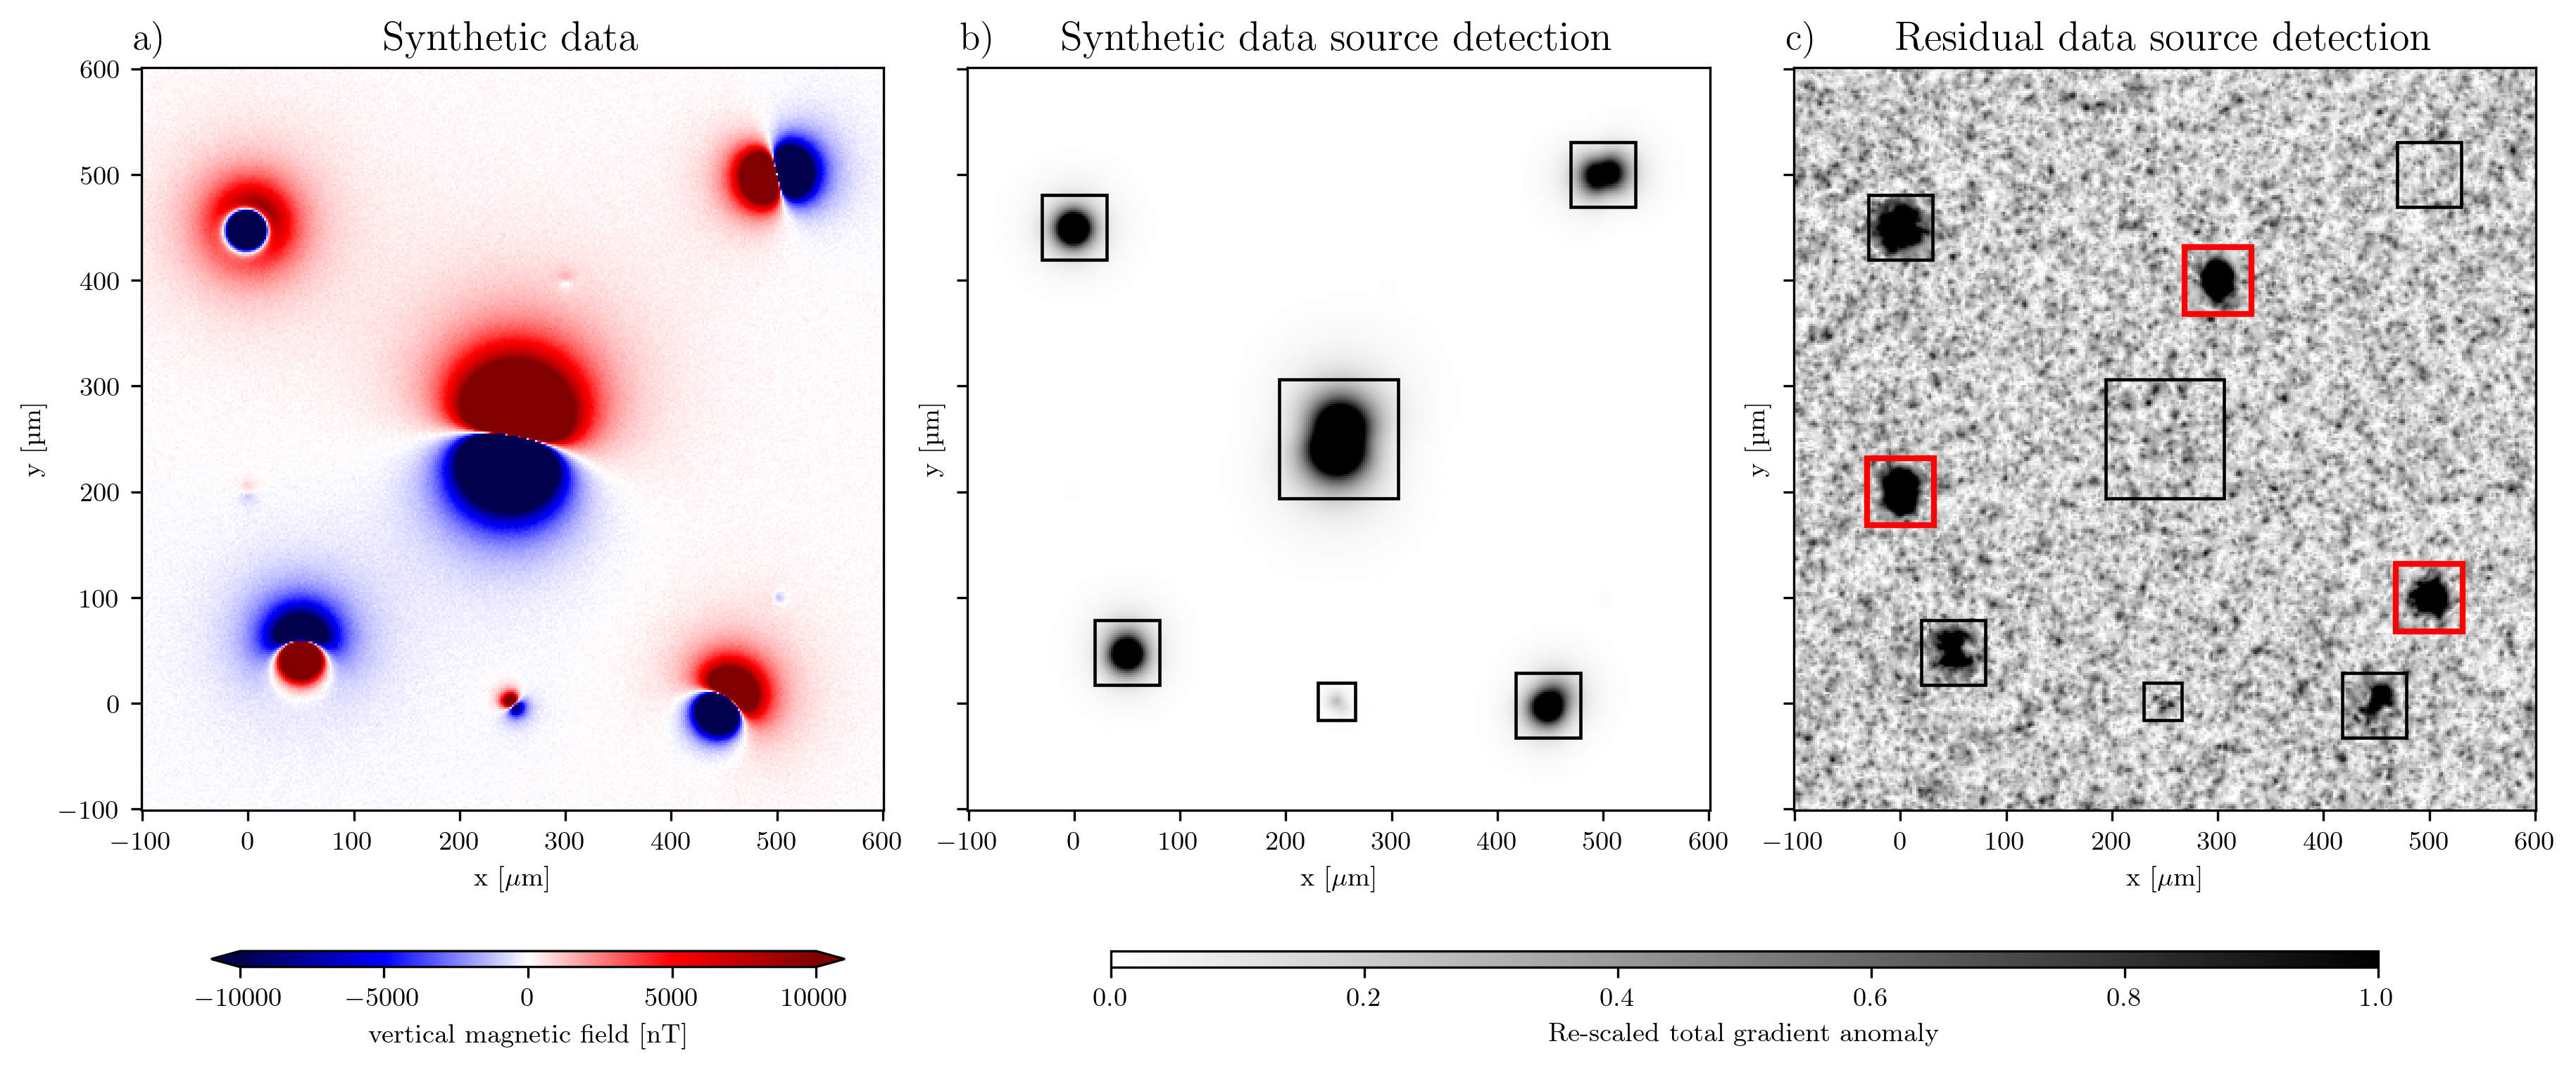
\includegraphics[width=1\linewidth]{paper/figures/re-detection-methodology.png}
      \caption{Source detection workflow on the residual anomaly. a) Synthetic sample featuring a wide range of magnetic moment intensities. b) The Blob detection algorithm identify the sources by using the total gradient obtained with the vertical component of the magnetic field. c) Result of the blob detection algorithm when applied to the total gradient of the residual anomaly.}
      \label{method-redetection}
    \end{figure}


%%%%%%%%%%%%%%%%%%%%%%%%%%%%%%%%%%%%%%%%%%%%%%%%%%%%%%%%%%%%%%%%%%%%%%%%%%%%%
\subsection{Criteria for Determining Magnetization Direction}

The selection of the magnetic moment direction of individual sources to achieve the total resultant moment of the sample followed a rigorous three-step methodology, designed to maximize accuracy and ensure the reliability of the results.

\subsubsection{Goodness-of-Fit Assessment}

The first step consisted of evaluating the goodness-of-fit by computing the coefficient of determination ($R^2$). This was done by comparing the real data with the residuals obtained from the developed model. A threshold of $R^2 \geq 0.90$ was empirically chosen, ensuring that at least 90\% of the data variance was explained by a dipolar model. This value provided a balanced trade-off between a stringent cutoff and the retention of a statistically significant dataset.

\subsubsection{Outlier Removal}

The second step involved the removal of outliers based on the logarithmic distribution of the magnetic moments ($\log_{10} M$). The magnitude of the magnetic moment was computed using the Euclidean norm:

\begin{equation}
    M = \| \mathbf{m} \| = \sqrt{m_x^2 + m_y^2 + m_z^2},
\end{equation}

where $m_x$, $m_y$, and $m_z$ are the Cartesian components of the magnetic moment. Outliers were identified using the interquartile range (IQR) method, following the principles of a boxplot:

\begin{equation}
    \text{Lower Bound} = Q_1 - 1.5 \times \text{IQR}, \quad \text{Upper Bound} = Q_3 + 1.5 \times \text{IQR},
\end{equation}

where $Q_1$ and $Q_3$ are the first and third quartiles, respectively, and $\text{IQR} = Q_3 - Q_1$.

\subsubsection{Jackknife Resampling}

In the final step we have applied a jackknife resampling technique to enhance the reliability of the vector distribution. To achieve statistical robustness, 50 iterations of the jackknife technique were performed. In each iteration, 20\% of the vectors were randomly removed. The final selected distribution was obtained by computing the median across all iterations:

\begin{equation}
    M_{\text{final}} = \text{median} \{ M_1, M_2, \dots, M_{50} \}.
\end{equation}

This approach ensured that the selected vectors were representative and minimally influenced by outliers or stochastic variations in the dataset, while still maintaining a sufficient number of data points for statistical accuracy.

%%%%%%%%%%%%%%%%%%%%%%%%%%%%%%%%%%%%%%%%%%%%%%%%%%%%%%%%%%%%%%%%%%%%%%
\section{Numerical Simulations}

In this section, we evaluate the effectiveness of the interfering sources method, in comparison with the method proposed by \citet{Souza-Junior2024}, by applying it to two synthetic datasets. The tests are structured as follows:  

\begin{enumerate}
    \item \textbf{Evaluating Overlapping Signal Detection:}
        This test simulates a single map containing both strong and weak sources to evaluate the the new methodology's effectiveness in discerning and accurately locating the weaker sources, despite the interferences causing by the from the stronger ones.
        
    \item \textbf{Assessing Performance with Variable Particle Density:}
    
        This test introduces a more complex scenario by simulating a specific magnetization direction for the magnetic sources. Additionally, three different particle density scenarios are modeled to test whether the method can reliably recover the magnetization direction across all cases.
        
\end{enumerate}

\subsection{Evaluating Overlapping Signal Detection}

The first model scenario consists of several dipole sources with varying moment magnitudes, inclinations, and declinations, organized into three distinct groups. The first group contains 150 dipoles with random orientations and moment magnitudes an order of magnitude larger than those in the second group. The second group comprises 50 dipoles with a stable orientation: an inclination of \(\ang{35}\) (\(\pm \ang{5}\)), a declination of \(\ang{340}\) (\(\pm \ang{5}\)), and dipole moment magnitudes centered at \(1.0 \times 10^{-16} Am^2\). Additionally, a third group includes 9 sporadic, deeper, and strongly magnetized sources with random orientations and significantly higher dipole moments of \(1.0 \times 10^{-11} Am^2\). Which totals 209 magnetic particles.

To evaluate the methodologies, we simulate these magnetic sources randomly distributed within a synthetic thin section measuring \(\qty{2000}{\micro\meter} \times \qty{2000}{\micro\meter}\). The synthetic vertical magnetic field data (\(b_z\)) are generated on a regular grid with \(\qty{2}{\micro\meter}\) spacing and a sensor sample distance of \(\qty{5}{\micro\meter}\), without any external applied field. Thus, the magnetic anomaly is solely caused by their dipole moment. High-frequency pseudo-random noise with a zero mean and a standard deviation of \(\qty{50}{\nano\tesla}\) is added for a realistic approximation of a QDM measurement \citep{Glenn2017}. The modeled sources were positioned at depths ranging from 1 to \(\qty{20}{\micro\meter}\). To further emulate actual acquisition conditions, a positive baseline shift of \(\qty{2000}{\nano\tesla}\) is applied to the magnetic field data. This setup tests the algorithm's robustness and accuracy when handling systematically shifted and noise-corrupted magnetic field measurements, as commonly observed in magnetic microscopy experiments.

The synthetic data inversion was resolved using both the standard method \citep{Souza-Junior2024} and the new proposed interfering sources methodology. A summary comparison of the classic Euler method and the iterative approach showed significant results in analyzing the synthetic data. The iterative Euler deconvolution method notably enhanced source detectability, with newly identified windows highlighted (green squares, Figure \ref{euler2}a). Figure \ref{euler2}b displays the 112 sources initially detected from the 209 modeled. Meanwhile, Figure \ref{euler2}c indicates that the iterative Euler method retrieved 165 sources. Initially, it may appear that the iterative method underperformed when compared to the standard in terms of tridimensional source location precision. Yet, most previously identified sources demonstrate reduced position misfit (barring sporadic deeper ones). The larger misfits in Figure \ref{euler2}c are linked to the newly identified grains (represented by the colored squares), as their smaller dipole moment results in greater error in the Euler estimation. This increase in accuracy is crucial, especially in scenarios where stronger magnetic sources can distort the magnetic field anomaly of weaker sources. Although this new methodology can markedly increase the accuracy in the estimated position for virtually all sources, the biggest errors are still related to clustered sources. Also, in both cases, the Euler deconvolution seems unaffected by the presence of a shift in the magnetic field.


\begin{figure}[tb!]
  \centering
  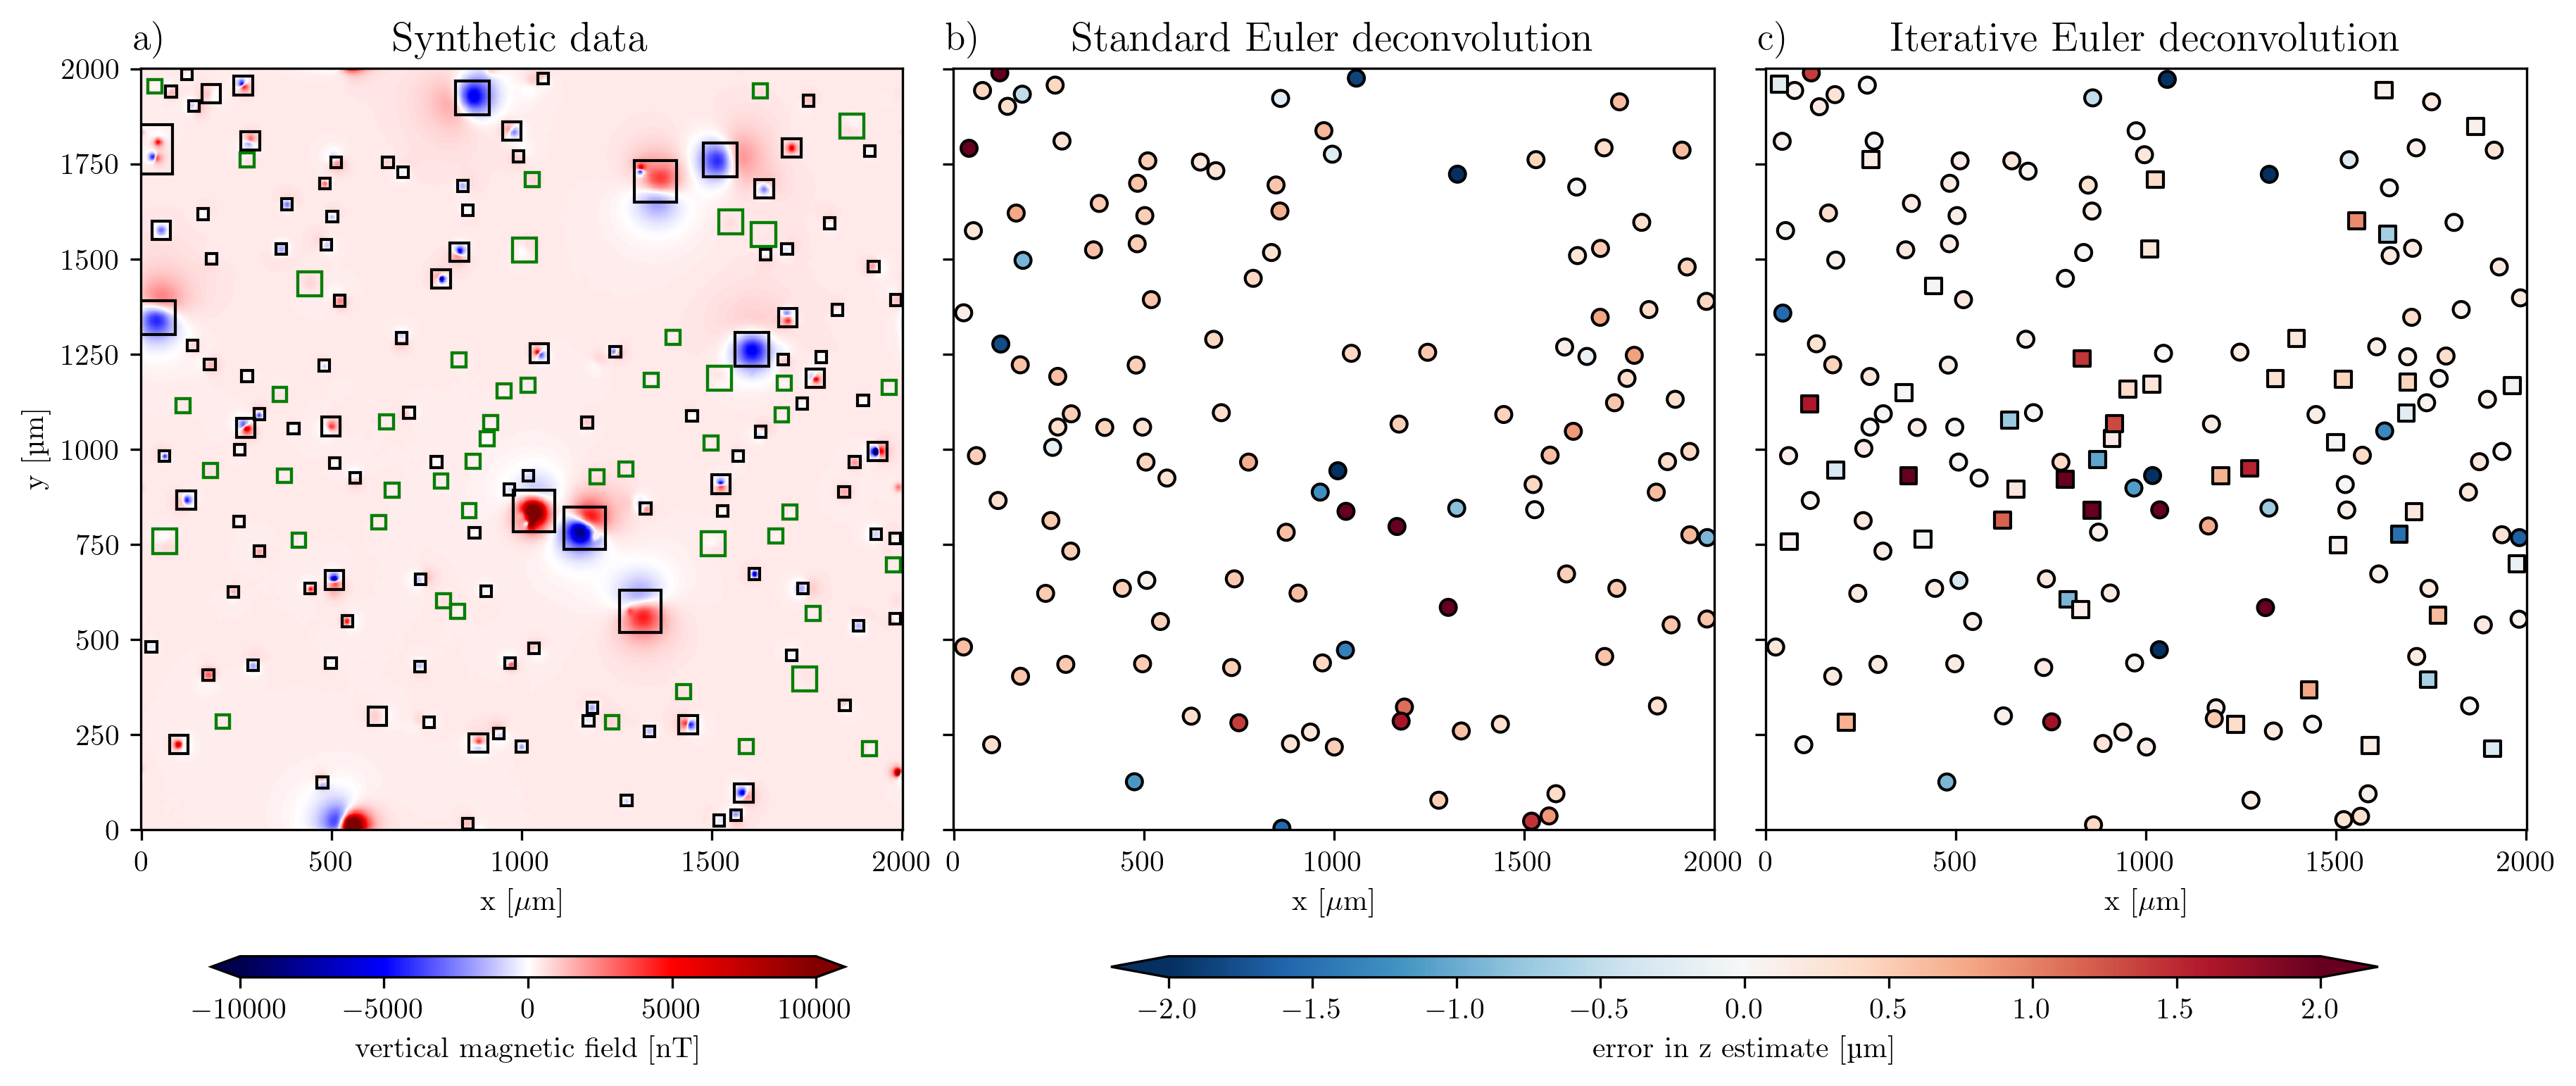
\includegraphics[width=1\linewidth]{paper/figures/euler-comparion-synthetic.png}
  \caption{
    Position estimation for the overlapping signals synthetic sample. (a) Initial detection window data for each magnetic source (black squares) and re-detection provided by the iterative solution (green squares). These data windows were used for the 3D position estimation of magnetic sources (colored circles) in the standard (b) and iterative (c) methodologies. Newly detected sources in the iterative method are represented as colored squares in panel (c).
  }
  \label{euler2}
\end{figure}

These iterative Euler estimated positions were used for the magnetic inversion due to their better results except for the standard method results, which were kept unchanged from the results presented by \citet{Souza-Junior2024}. Figure~\ref{inversion2} presents a comparison of the estimated magnetic moment directions for the standard (Figure~\ref{inversion2}b) and iterative (Figure~\ref{inversion2}c) methods, in relation to the true directions (Figure~\ref{inversion2}a). As expected, the iterative method provides a better overall agreement with the true directions, recovering a larger number of sources with reliable estimates. The improvement is particularly noticeable as the iterative approach is capable of identifying signals from weaker particles, increasing the number of recovered sources. This has the potential to improve the statistical robustness of the estimated directions, making the method particularly useful for applications in magnetic microscopy.


\begin{figure}[tb!]
  \centering
  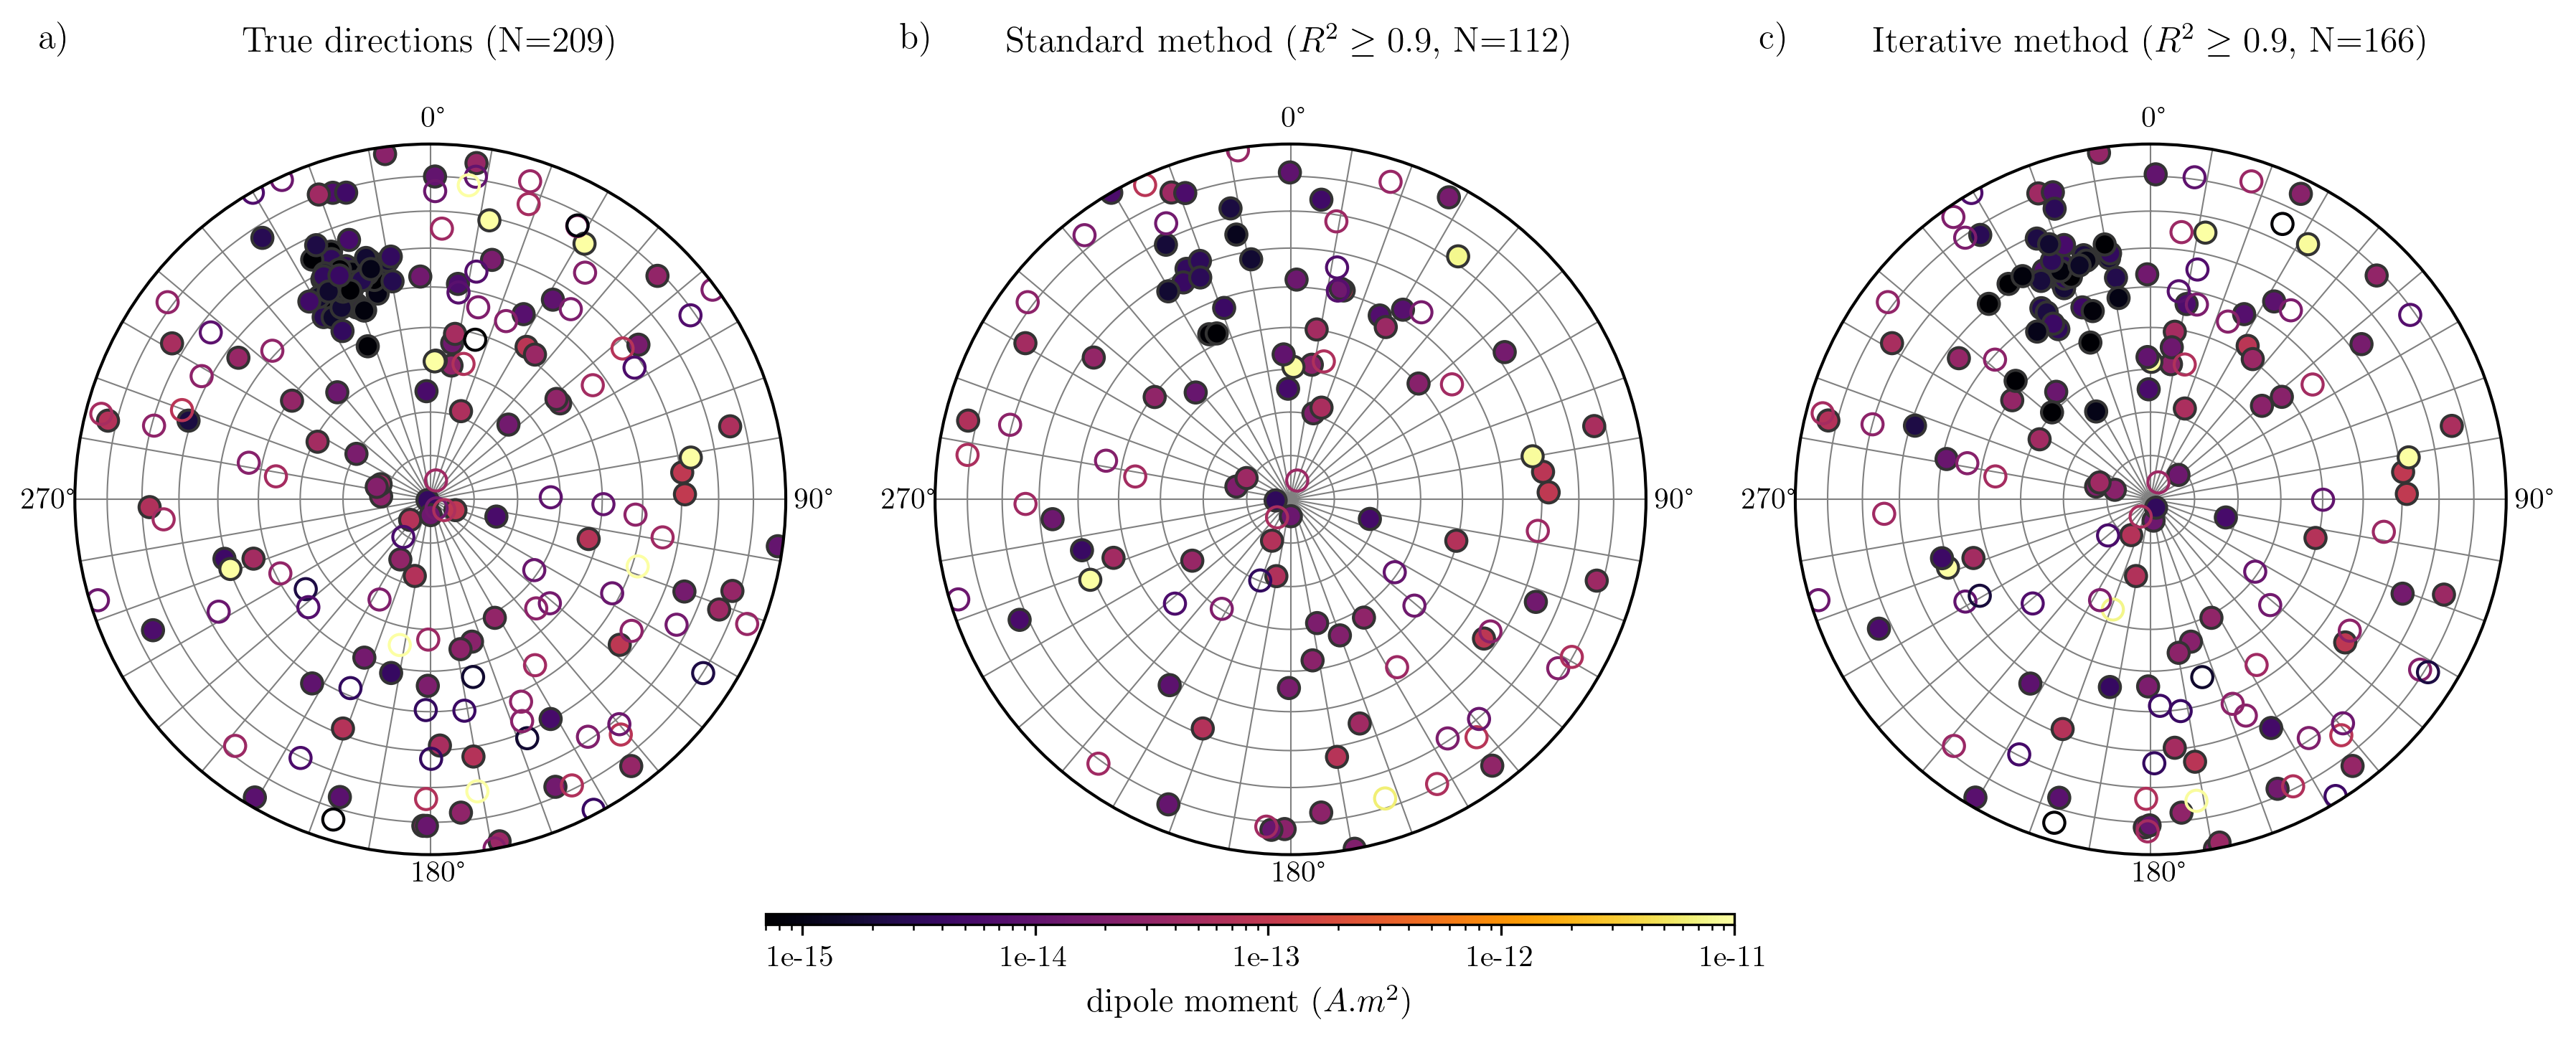
\includegraphics[width=1\linewidth]{paper/figures/synthetic-data-stereograms-comparison.png}
  \caption{
    Comparison of true and estimated dipole magnetic moments and directions for the overlapping signals in the synthetic sample. Panel (a) shows the true modeled direction, while panels (b) and (c) display the estimated vector directions obtained using the standard ($M = 112$) and iterative ($M = 165$) methods, respectively. Results for both methods were filtered based on the coefficient of determination ($R^2 \geq 0.9$). Directions are hued by magnitude of their magnetic moments. Open/closed circles indicate positive/negative inclinations.
  }
  \label{inversion2}
\end{figure}



\subsection{Assessing Performance with Variable Particle Density}

To assess the impact of particle density on the simulated results, three different grain distributions were considered, with \(N=500\), \(N=1000\), and \(N=2500\), corresponding to grain densities of approximately \(9000\), \(18000\), and \(45000\,\mathrm{grains/mm^3}\), respectively. These densities were chosen to numerically simulate concentrations expected in different rock types. Lower densities are typical of rocks with scarce magnetic grains, like carbonates, while the highest density approximates rocks with higher particle concentrations, such as basalts.

The directional parameters and magnetic moment intensities distributions were kept constant across all simulations, as the goal was to isolate the effects of increasing particle density. For each simulation, the total \(N\) magnetic dipole sources were created and randomly distributed across a thin section of \qty{2000}{\um} \(\times\) \qty{1400}{\um}. The dipole moments were sampled from a lognormal distribution centered at a mean amplitude of \(1 \times 10^{-14}\,\mathrm{A \cdot m^2}\), with a standard deviation spanning two orders of magnitude. This configuration ensures that most of the distribution is concentrated around the mean, while also allowing for the presence of particles with magnetic moments as strong as \(10^{-11}\,\mathrm{A \cdot m^2}\), simulating larger particles with a greater influence on the magnetic field compared to weaker particles. The modeled sources were also positioned at pseudo-random depths ranging from 1 to \(\qty{20}{\micro\meter}\).

A variety of geological processes can lead to the acquisition of natural remanent magnetization (NRM). If the NRM is primary—formed at the same time as the rock—it will generally align with the ambient magnetic field, such as a planetary field. However, the alignment of individual grains is influenced by multiple factors, including particle properties \citep[shape, size, domain state,][]{Bellon2025} and the conditions under which NRM is acquired, such as the cooling rate of lavas. As a result, while individual grain signals may show a general tendency toward alignment, the magnetic moments of many particles will still exhibit some degree of random orientation. To mirror this variation in our synthetic data, we set the inclination and declination of directional parameters primarily at 30° and 330°, respectively. A 50° dispersion angle introduced variability within spherical statistics, where directional data extends over a unit sphere rather than Cartesian coordinates. This angle indicates a broad spread of directions around the mean, accounting for significant variability in dipole directions, which is crucial for accurately representing the natural diversity of magnetic sources.

The synthetic magnetic field \(b_z\) was computed over a grid with a \qty{2}{\um} spacing, and the measurement plane was set at a constant height of \qty{5}{\um} above the thin section. High-frequency pseudo-random noise, following a Gaussian distribution with zero mean and a standard deviation of \qty{50}{\nano\tesla}, was added to the computed field to mimic realistic measurement conditions. Additionally, a pseudo-random baseline shift ranging from \(-2000\) to \(2000\,\mathrm{nT}\) was introduced to replicate the acquisition process in magnetic microscopy. The simulations were conducted in a zero external field environment, where all signals generated in the maps were solely and exclusively caused by the magnetization of the simulated particles, simulating real acquisitions typically performed in magnetically shielded rooms to eliminate the influence of the Earth's geomagnetic field. A total of 10 simulations were carried out for each different particle density level. The resulting magnetic field data were exported to NetCDF format for further analysis.


\begin{figure}[tb!]
  \centering
  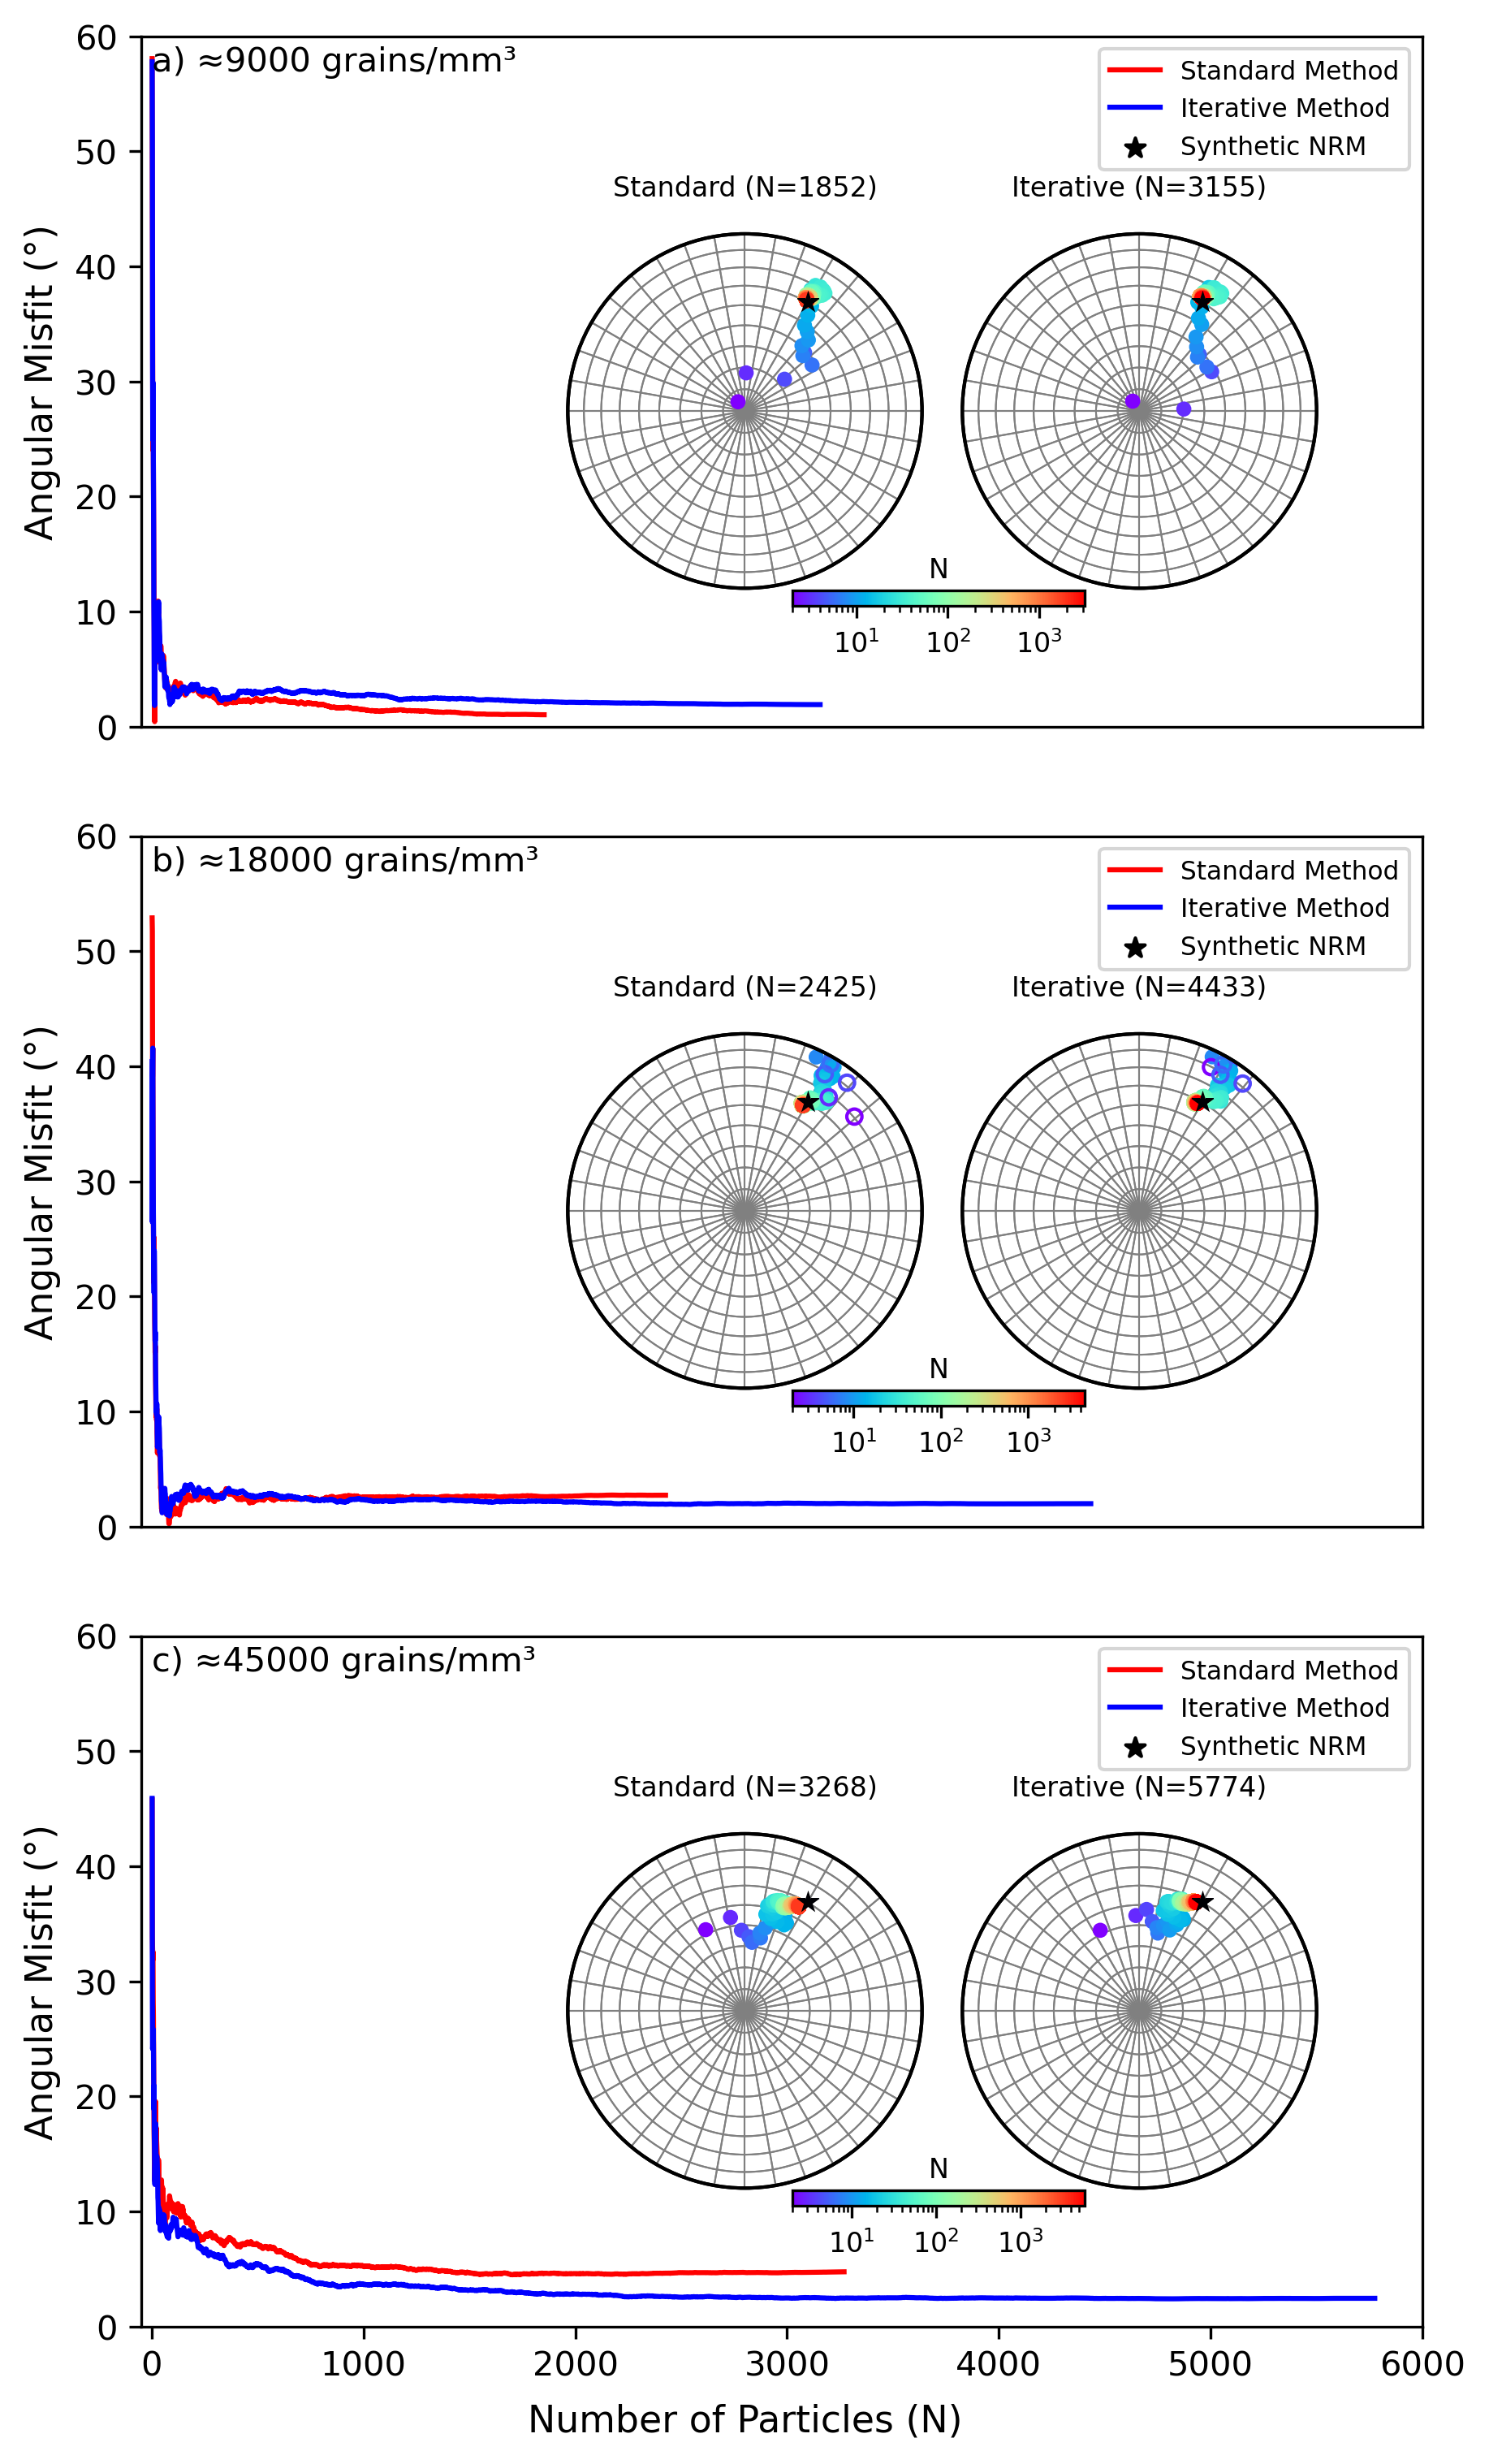
\includegraphics[width=0.7\linewidth]{paper/figures/synthetic-different-densities-stereoplot.png}
  \caption{
blablabla
  }
  \label{synthetic-data-stereograms}
\end{figure}


\section{Real Data Application}

After demonstrating the applicability of the new methodology through the numerical simulations, we applied it to real SMM data. We can rely on rocks carrying a thermoremanent magnetization (TRM) to test out our method, as they represent most of the robust paleomagnetic records. The magnetic particles \citep[most commonly magnetite,][]{OReilly1984} acquire TRM as they cool below their Curie temperature, with the magnetization direction becoming "locked in" upon reaching the blocking temperature \citep{Dunlop1997}. When grains are sufficiently small and exhibit homogeneous, unidirectional magnetization (single domain, SD), the acquisition and preservation of magnetic signals are physically supported by Néel’s theory \citep{Neel1949, Neel1955}. This allows them to retain remanent magnetization for billions of years, making them excellent recorders of the paleomagnetic field. In addition to SD particles, pseudo-single domain (PSD) particles—characterized by flower and vortex states—are also stable and can preserve magnetization for timescales comparable to the age of the Solar System \citep{Nagy2017, Lascu2018,Bellon-2024a}. Conversely, Néel’s theory does not apply to larger particles (multidomain, MD), which have unstable remanent magnetization \citep[e.g., due to viscous domain reorganization,][]{DeGroot2014}, limiting their capacity to reliably record the geomagnetic field. 

In this section, we worked with two distinct TRM-bearing samples. The NRM of the samples was measured using the 2G RAPID Superconducting Rock Magnetometer at the Harvard Paleomagnetics Lab, Department of Earth and Planetary Sciences, Harvard University. As a result, the measurements encompass both the primary TRM and any possible viscous components acquired through the natural magnetic relaxation of some particles. Additionally, to ensure consistency between the magnetometer measurements, which were taken vertically, and the maps produced with the QDM, it was necessary to apply a 90-degree clockwise rotation around the \textit{x}-axis to the vertical measurements. This rotation ensures that both measurements are in the same reference frame.

\begin{enumerate}
\item \textbf{Evaluation with a Stable Assembly:}

The first test focuses on the analysis of a thin-section of an archaeological ceramic sample. This sample is characterized by a mid-term density of magnetic particles, with most of them falling into SD and PSD categories. The goal of this test is to assess the method’s performance in real samples where the magnetic carriers are stable, and the influence of unstable domains is minimal. This setting allows for a clear evaluation of the methodology’s sensitivity and accuracy when working with well-defined magnetic signals.

\item \textbf{Evaluation with a Complex Densely Packed Assembly:}
The second test involves the examination of the basaltic rock sample. This sample acquired its TRM during the natural cooling process of lava, leading to a high density of magnetic particles. Unlike the ceramic sample, the basalt is significantly influenced by unstable MD particles, which introduce additional complexity to the magnetic signal. The aim of this test is to verify the method’s effectiveness in identifying and analyzing magnetic sources in challenging conditions, where densely packed magnetic carriers and the presence of unstable remanent magnetization could affect the reliability of the results. This contrast presents a more complex scenario, challenging the methodology to accurately identify and interpret magnetic sources in samples with densely packed and less stable magnetic carriers.
\end{enumerate}


\subsection{Evaluation with a Stable Assembly}

To evaluate the feasibility of magnetic microscopy techniques in detecting and characterizing TRM, we selected a well-preserved fragment of baked clay pavement tile (sample RSLG1) from the archaeological site São Luiz Gonzaga reduction (1657-1687 AD). This fragment was collected by \citet{Poletti2016} and was subsequently used in a paleointensity study. According to the same authors, the magnetic properties of the sample indicate that magnetization is carried by a low-coercivity phase, most likely PSD Ti-poor titanomagnetite. Their interpretation is supported by the isothermal remanent magnetization (IRM) curves saturated at fields up to approximately 0.3 T, narrow hysteresis loops, and maximum NRM demagnetization temperatures around 550°C. First order reversal curves (FORC) also confirm a predominance of non-interacting SD/PSD grains. These characteristics make the sample an ideal candidate for magnetic microscopy studies aimed at investigating its natural remanent magnetization.

In this study, the vertical component of the magnetic field ($b_z$) was scanned directly from the NRM of the sample using the Quantum Diamond Microscope (QDM) at the Harvard Paleomagnetics Lab (Department of Earth and Planetary Sciences, Harvard University). A total of 20 randomly selected regions were subjected to this scanning procedure to ensure representative coverage of the sample's magnetic properties. The scanned area measured $\qty{1410}{\um} \times \qty{2256}{\um}$ with a grid spacing of \qty{2.35}{\um} ($N = 576 \times 10^{3}$). Data acquisition was conducted at a constant sensor-sample distance of \qty{5}{\um} in a background magnetic field of $< \qty{1}{\micro\tesla}$, provided by the magnetically shielded room. This allowed for high-resolution mapping of the magnetic field distribution.

We have applied both the standard and iterative algorithms to this data, and all magnetic vectors associated with the identified particles were compiled into a database. This dataset was filtered based on the model's coefficient of determination ($R^2$), with only vectors meeting the criterion of $R^2 \geq 0.9$ being retained. The selected vectors were then ordered by intensity and progressively summed. At each step, the cumulative vector was compared with the NRM measured of the whole sample (which was acquired with a rock magnetometer, see the Methodology section for more details).

The comparison between the standard and iterative algorithms highlights significant differences in their ability to reconstruct the NRM of the sample. As shown in Figure~\ref{ceramic-data-stereograms}, the angular misfit between the cumulative magnetic vector and the measured NRM decreases more effectively with the iterative approach. While the standard method results in a consistently higher misfit, stabilizing around \ang{55}, the iterative method quickly refines the alignment, reducing the misfit to approximately \ang{10} within a few hundred particles. This indicates that the iterative approach is more efficient in capturing the true remanent magnetization with fewer contributing grains. The stereographic projections further support this observation by illustrating the directional distribution of the filtered vectors for each method, where the iterative approach yields a distribution more closely aligned with the measured NRM (star symbol) and the jackknife mean direction (square symbol). These results demonstrate that the iterative method significantly enhances the accuracy of NRM reconstruction by effectively mitigating directional dispersion.

The limited improvement threshold in directional accuracy, even as more particles are added, is a noteworthy observation that we can only hypothesize about. We propose two possible contributing factors. First, as previously discussed, only a fraction of the magnetic grains are fully aligned with the magnetic field. When measuring the total NRM at the macroscopic scale, the contributions of all grains are summed, allowing randomly oriented signals to cancel out while the more aligned grains enhance the overall alignment with the field direction. Classical rock thin sections, like the one used in this study, are typically prepared at a thickness of around \qty{30}{\um} to facilitate the identification of mineral features under a petrographic microscope. Within such a thin section, millions of magnetic minerals are likely present. However, in SMM data acquisition, we only sample a small portion of the entire thin section. Even within this measured area, not all magnetic signals are fully detected, as the measured magnetic moment depends on both the depth of the particles and their magnetic strength. As a result, when more particle directions are incorporated into the combined magnetic signal, a saturation effect may occur. Beyond a certain threshold, the inclusion of additional, randomly oriented signals could outweigh the contribution of well-aligned grains, limiting further improvement in directional accuracy. This would explain why, despite increasing the number of particles, the expected refinement in the reconstructed direction is not observed.

The second hypothesis involves human-induced errors during the measurement process. The sample had to be manually positioned and oriented in both the QDM and the 2G magnetometer, introducing potential sources of misalignment. In the 2G magnetometer, the sample was measured in a vertical orientation and later rotated to match the reference frame of the thin section used in the QDM analysis. This manual handling and reorientation may have introduced small but cumulative misalignments, contributing to the observed directional discrepancies.

\begin{figure}[tb!]
  \centering
  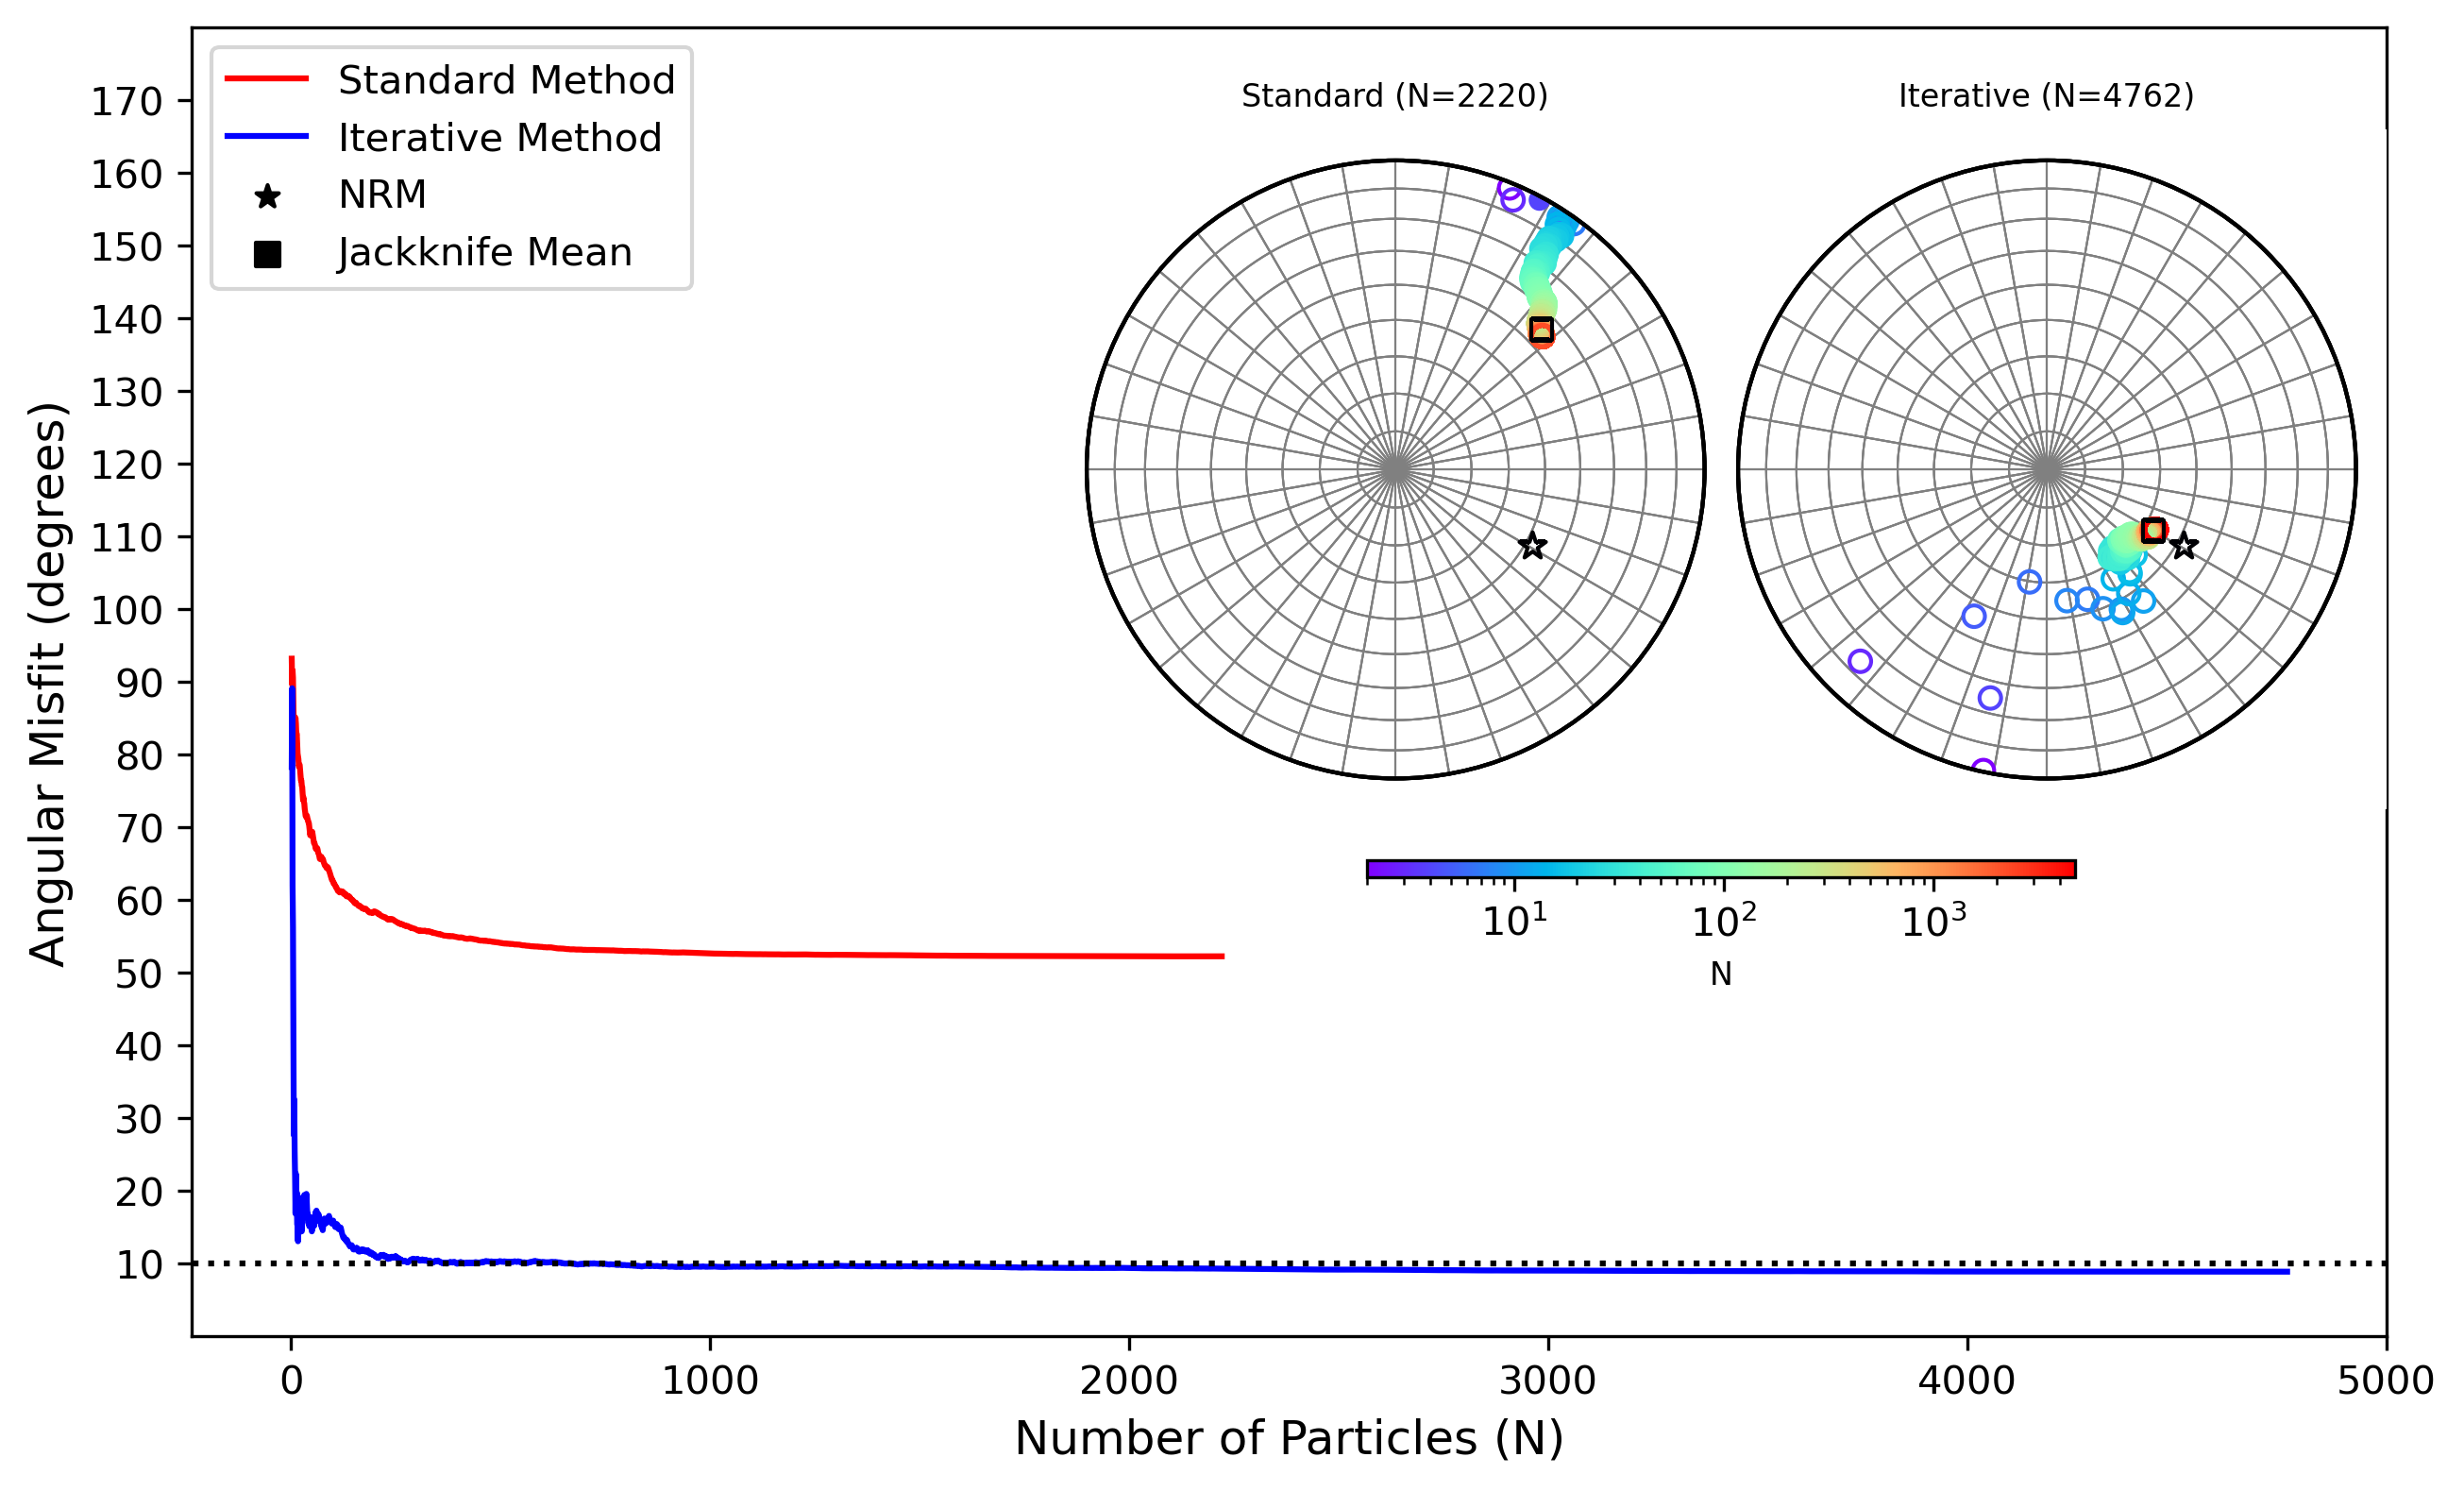
\includegraphics[width=1\linewidth]{paper/figures/ceramic-data-stereoplot.png}
  \caption{
  Comparison of the standard (red) and iterative (blue) algorithms in reconstructing the NRM direction from the ceramic sample. (Left) Angular misfit between the cumulative vector and the measured NRM as a function of the number of particles ($N$). (Right) Stereographic projections of the filtered magnetic vectors ($R^2 \geq 0.9$) for both methods, with the measured NRM (star) and the jackknife mean (square) indicated. The color gradient denotes the logarithmic scale of particle counts, with warmer colors representing higher concentrations.
  }
  \label{ceramic-data-stereograms}
\end{figure}

%%%%%%%%%%%%%%%%%%%%%%%%%%%%%%%%%%%%%%%%%%%%%%%%%%%%%%%%%%%%%%%%%%%%%%%%%%%%%%%
\subsection{Evaluation with a Complex Densely Packed Assembly}

In order to apply our method to a more magnetically complex sample, we have chosen a basalt from the Caviahue-Copahue volcanic complex (Argentina), specifically a core from the Cola de Zorro Formation (COP01) \citep{Moncinhatto2019}. The lithotypes of this geological formation present a flow-aligned fabric, specially marked by plagioclase crystals, but also containing both phenocrysts and smaller crystals in the matrix, exhibiting a trachytic texture. Its magnetic mineralogy is mainly composed of low-Ti magnetite, with most macroscopic crystal sizes ranging from 10 to 50 \si{\micro\meter} \citep{Moncinhatto2019}. This size distribution is reflected in the high-field experiments, including IRM acquisition curves, hysteresis loops, and FORC diagrams. They reveal saturation at fields around 0.2 \si{T}, coercivities below 10 \si{mT}, and the FORC diagrams are typical of multidomain (MD) grains. Nonetheless, other samples within the same formation display coercivities between 10 and 20 \si{mT} and FORC diagrams characteristic of magnetite with a PSD behavior, or mixtures of SD and MD grains.

The acquisition of QDM data was essentially the same as the aforementioned experiment with the ceramic tile. The QDM scans were performed to capture the magnetic field distribution at high spatial resolution. To better compare the results with the tile sample, the same number of randomized mapping spots was performed. The resulting data enabled the calculation of angular misfit as a function of the number of particles, providing insight into the reliability of different analytical methods.

The results reveal a clear difference in the performance of the standard and iterative methods in reconstructing the NRM direction. As shown in Figure~\ref{basalt-data-stereograms}, the iterative method consistently achieves lower angular misfit values as more particles are incorporated, demonstrating improved accuracy and stability. In contrast, while the standard method also reduces the misfit over time, it stabilizes around 10 degrees only after approximately a thousand grains, with a broader dispersion of directional data. The stereographic projections further illustrate these differences. The standard method exhibits a wider spread of vectors, suggesting that many individual particle contributions remain misaligned. Meanwhile, the iterative method results in a more tightly clustered distribution, with the misfit tending toward zero as the number of particles increases (although there is also, seemingly, a stagnation threshold). This suggests that the iterative approach is more effective in refining the directional signal, leading to greater precision in the reconstructed magnetization. 

\begin{figure}[tb!]
  \centering
  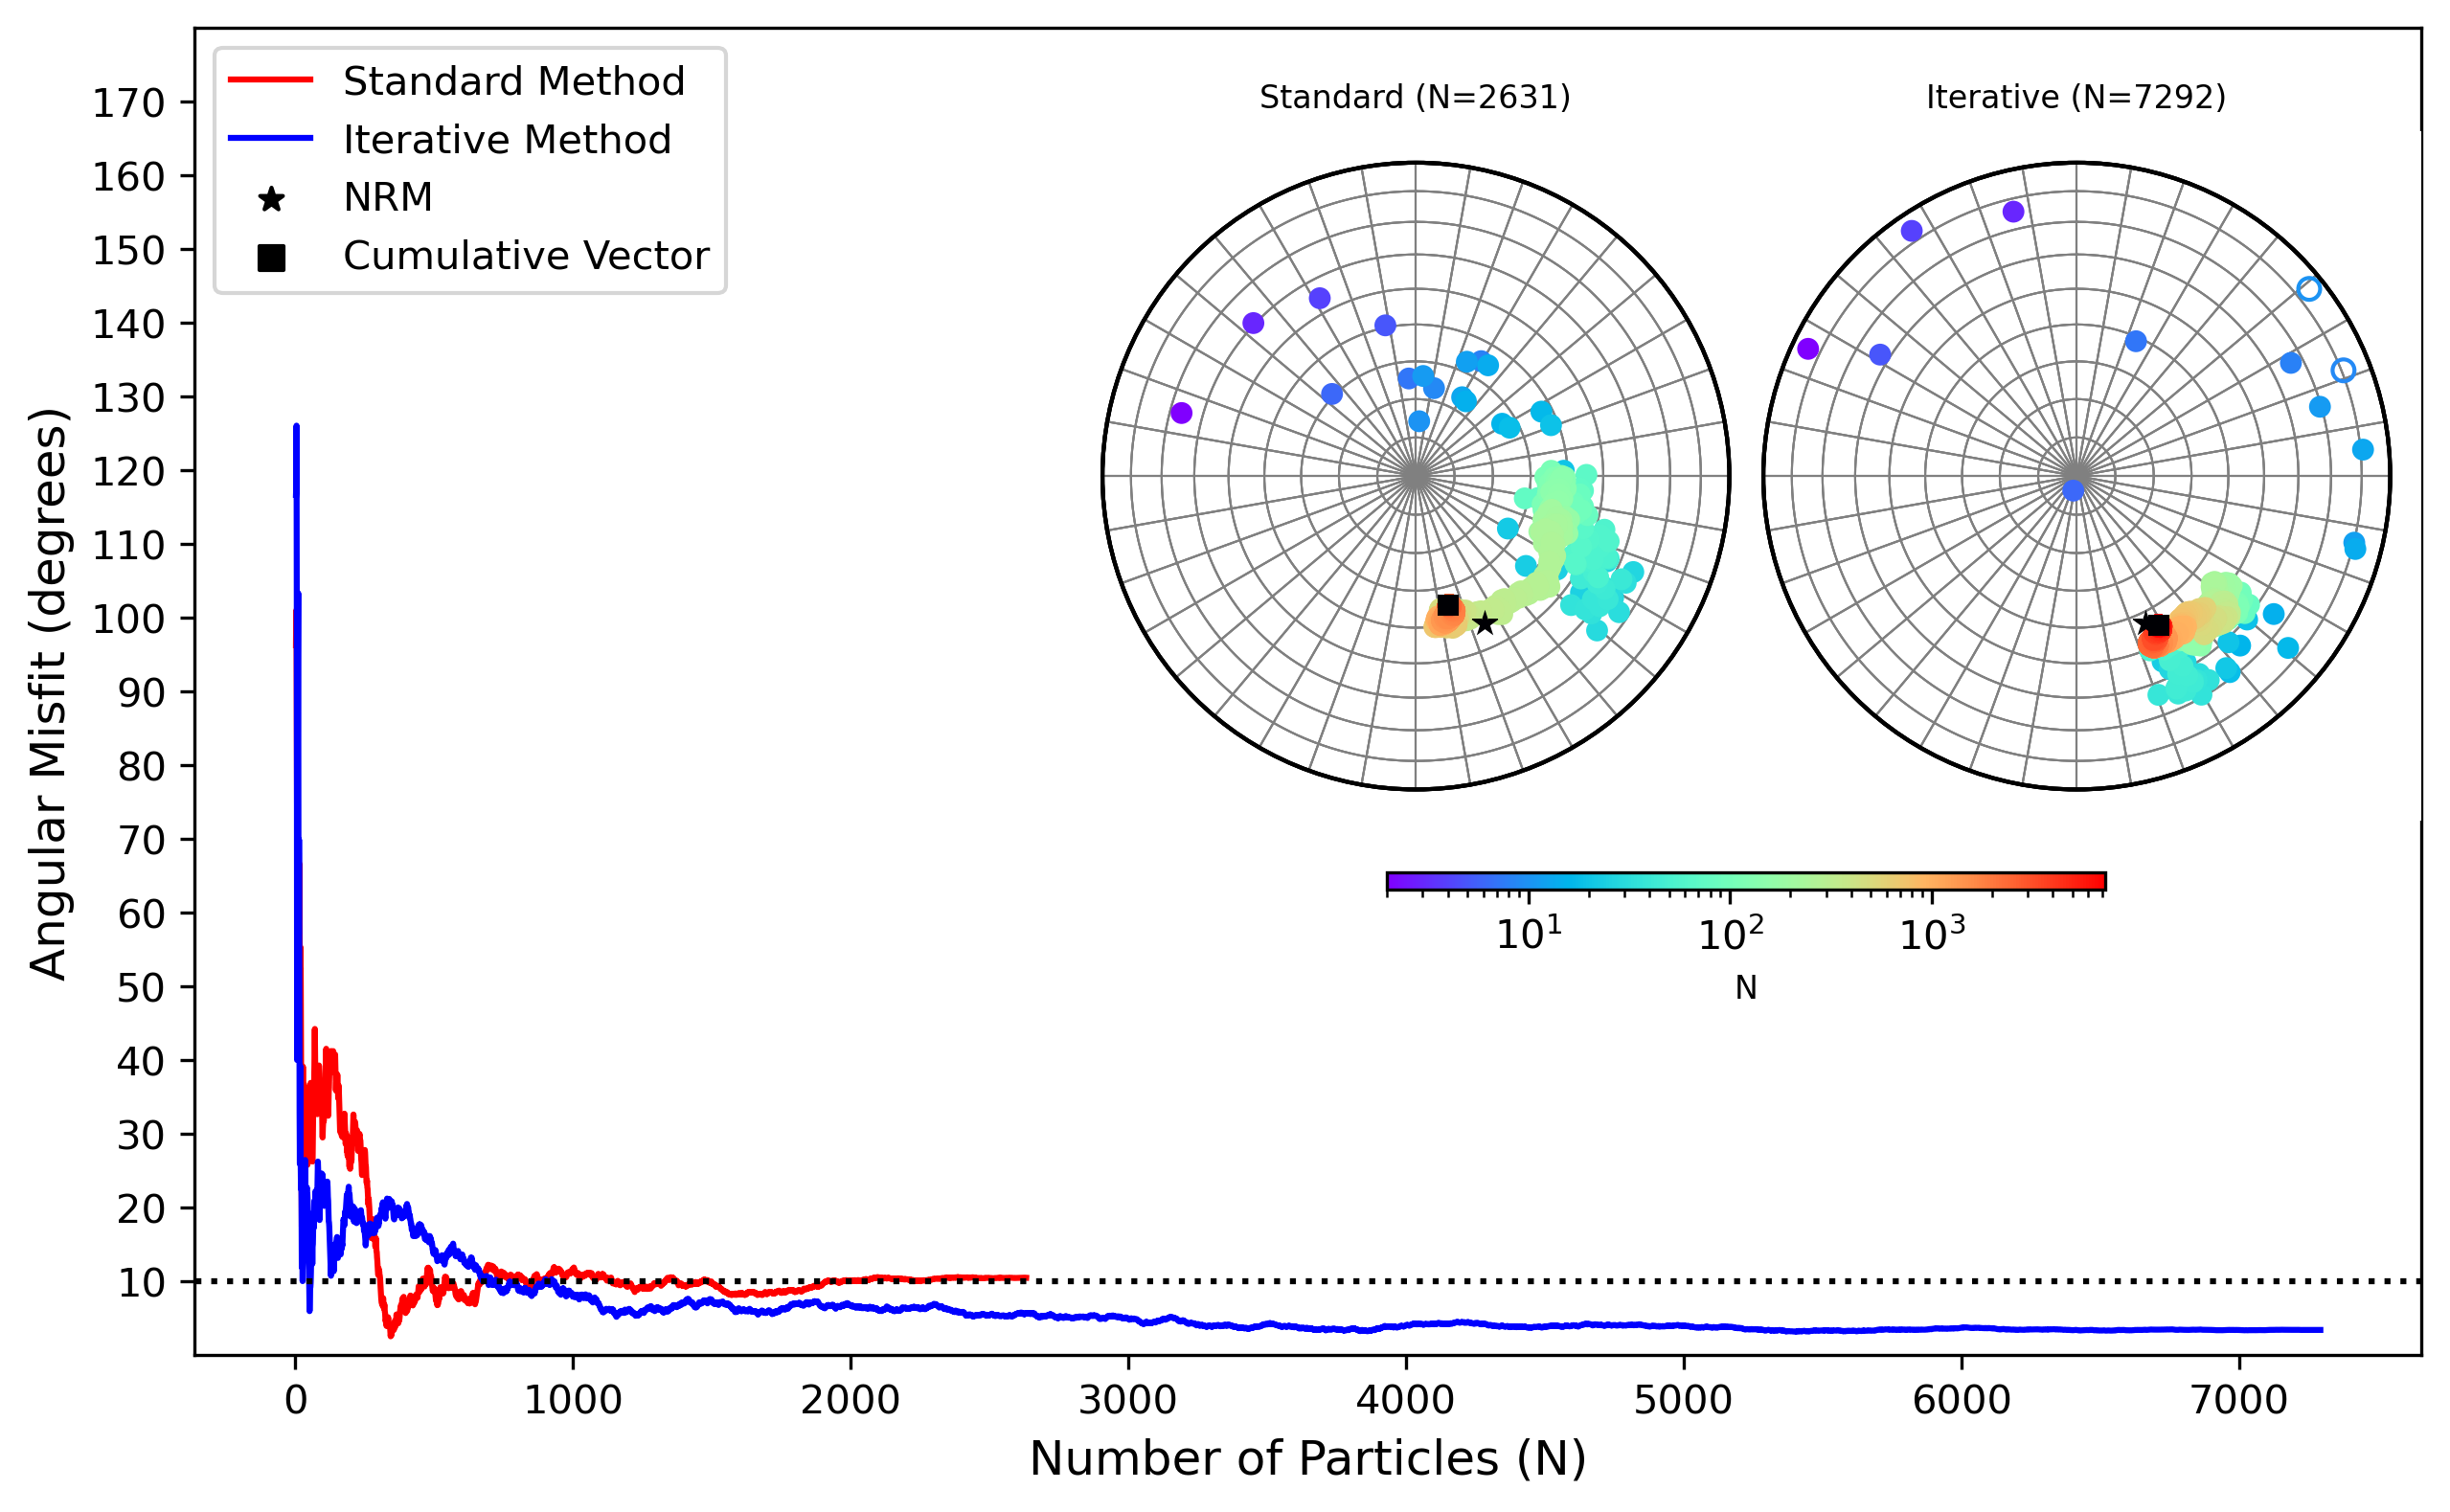
\includegraphics[width=1\linewidth]{paper/figures/basalt-data-stereoplot.png}
  \caption{
  Comparison of the standard (red) and iterative (blue) algorithms in reconstructing the NRM direction from the basalt sample. (Left) Angular misfit between the cumulative vector and the measured NRM as a function of the number of particles ($N$). (Right) Stereographic projections of the filtered magnetic vectors ($R^2 \geq 0.9$) for both methods, with the measured NRM (star) and the jackknife mean (square) indicated. The color gradient denotes the logarithmic scale of particle counts, with warmer colors representing higher concentrations.
  }
  \label{basalt-data-stereograms}
\end{figure}

%%%%%%%%%%%%%%%%%%%%%%%%%%%%%%%%%%%%%%%%%%%%%%%%%%%%%%%%%%%%%%%%%%%%%%%%%%%%%%%
\section{Discussion}

Inverting unique magnetic moment from SMM data, regardless of the technique, demands knowing the position of sources. The application of the Euler deconvolution technique emerges to avoid additional measurements, such as nano-tomography, to uncover that information. The isolated windows approach, as justified by \cite{Souza-Junior2024}, enables the separation of the primary signal from the surrounding area using the total gradient anomaly. This method effectively isolates the desired signal while excluding regions outside the window boundaries, which are less sensitive to variations in the magnetic parameters of the specific source. Using this windows approach enables a rapid solution to the inversion problem while keeping it largely overdetermined, since only three parameters are solved per sliced data. However, this thresholding exclusion of the area from the inversion domain violates the basic theory of inversion, which demands that the entire system be considered, ensuring that the interactions between all sources are properly accounted for to obtain a unique and precise solution \citep{Baratchart2013, Lima2013}. Thus, the previous approach of \cite{Souza-Junior2024} will not yield reliable results in all cases. Specifically, in cases influenced by distant sources, even those that are weak, either within the window or close by, which compromises its effectiveness. The latter reflects on a higher amount of results discarded by the filtering criterion. 

To tackle these challenges, the iterative method was introduced, providing a more reliable solution for mitigating interference between sources while still preserving the isolated windows approach. Naturally, this comes at the cost of increased inversion time, but the method remains efficient enough to run on a personal computer without demanding massive computational power. Despite the improvements, not all problems have been solved. The new method is more effective at detecting particles and results in more particles passing through the filtering criteria. However, it still faces challenges with inherent limitations of the Euler deconvolution, such as clustered signals. This introduces position estimation errors that are directly influenced by the particle's magnetic signal strength. In particular, errors in vertical positioning lead to a compensatory trade-off between this positional uncertainty and the recovered dipole intensity. For this reason, our focus here is on the directional aspects of the dataset, while the intensity aspect will require more complex future experiments, along with the implementation of a more refined approach to solving Euler's homogeneity equation, as proposed by \citet{Uieda2024}.

\subsection{Directional Recovery Assessment}

As noted by \citet{Oliveira2015Estimation}, the least-squares estimator is less sensitive to small errors in particle position when recovering directional information (declination and inclination). This makes the new method particularly effective in refining estimates, increasing the number of results that meet the filtering criteria. As a result, the approach becomes more statistically robust, ultimately improving the overall data quality. The fitting performance was assessed using both synthetic and real datasets, requiring a reliable reference for comparison. In the case of synthetic data, a directional bias (synthetic NRM) was introduced to the dipole magnetic moments based on a spherical distribution. For real samples, the reference direction was obtained from NRM measurements of the whole thin-section using the 2G magnetometer.

From the synthetic tests (Figure~\ref{synthetic-data-stereograms}a-c), both the original \citep{Souza-Junior2024} and iterative methods performed well in recovering the directional bias, mainly for two reasons. First, dipolar models are generally simpler and tend to produce more results that pass the filtering criteria. Even though the standard method is less efficient in estimating parameters, this deficiency is compensated by the overall behavior of the synthetic sample, and any poor-fitting is treated as random inputs that are effectively removed in the vector sum. The second reason is that, despite a wide distribution of particle moments (from \(10^{-15}\) to \(10^{-11}\)), the stronger particles, which could have further complicated the signal, also followed the bias direction. This contrasts with the overlapping signals synthetic case, where the strong particles were randomly oriented. Nonetheless, it serves as a proxy to isothermal remanent magnetization study cases.

For the real samples, the results deviated from initial expectations. The most stable assembly, characterized by a higher proportion of SD/PSD grains and a lower packing density of magnetic particles, exhibited the highest angular misfit, though it remained below 10 degrees (Figure~\ref{ceramic-data-stereograms}). In contrast, the basalt sample produced an angular misfit of less than 5 degrees (Figure~\ref{basalt-data-stereograms}), a result that was not anticipated given the high particle density, particularly the presence of MD grains. This density violates a key assumption of the method, namely that each window should ideally contain a single particle \citep{Souza-Junior2024}. A possible explanation for this positively surprising behavior is provided by recent nanotomography studies of basaltic rocks \citep[\textit{e.g.}][]{Out2024, Out2025}, which have revealed clusters of magnetic particles smaller than \(1~\mu m\). When a window captures such a cluster, the recorded signal represents the sum of the individual contributions. If the cluster exhibits a directional bias, this bias is likely to be reflected in the inversion result. This effect may also account for the improved performance of the standard method in the basaltic sample. While this approach does not effectively resolve interfering sources, it can still capture the overall directional bias of clustered particles, resulting in a lower angular misfit despite the sample’s high particle density.


\subsection{Empirical Insights for Paleomagnetic Studies}

\citet{Berndt2016} established a critical baseline by estimating that at least 10 million particles are required to obtain stable directions using magnetic microscopy data. However, this estimate has, to date, posed significant challenges for the application of magnetic microscopy in paleomagnetic studies. While their work is mathematically rigorous, certain assumptions may contribute to an overestimation of the required number of particles. One key factor in this overestimation could be the role of \textit{$\alpha_{95}$}, which scales the number of required particles to extreme values. Notably, their formulation primarily considers uniaxial anisotropy in spherical SD particles, whereas these grains, in reality, should exhibit multiaxial anisotropy. Additionally, the inclusion of vortex-state (PSD) particles was handled through a purely analytical approach to adjust the magnitude of magnetization, as these particles cannot be fully resolved analytically. These considerations suggest that while their estimate provides an important theoretical reference, it may not accurately reflect the number of particles required under more realistic conditions.

A major shift in perspective occurred nearly a decade later with the work of \citet{Bellon2025}, which revisited TRM acquisition studies using vortex-state particles under various conditions. This study built upon the now well-established understanding that vortex-state particles constitute the dominant carriers of stable paleomagnetic signals in igneous rocks. In this new approach, different particle morphologies—and consequently distinct anisotropies—were considered, and micromagnetic simulations were employed to estimate blocking temperatures and the associated energy distributions of domain states that could be accessed during TRM acquisition \citep{Bellon2025}. Their simulations, which also explored a range of possible field intensities, revealed that for fields exceeding approximately $2 \mu \text{T}$, the number of particles required to obtain a reliable direction with minimal angular misfit to the field is of a few thousand.
 
Thus, our present work provides empirical support for these numerical predictions. As shown in Figures~\ref{ceramic-data-stereograms} and \ref{basalt-data-stereograms}, slightly more than a thousand grains were sufficient to achieve a misfit below 10 degrees. For the ceramic tile sample, paleointensity measurements from a sister sample, as reported by \citet{Poletti2016}, yielded an average intensity of $40.2 \pm 2.4\ \mu\text{T}$ (dated to 1657–1687 AD). This aligns with the findings of \citet{Bellon2025}, which suggest that higher field intensities facilitate more accurate TRM acquisition with fewer magnetic carriers. Similarly, in the basalt samples, a few thousand grains were sufficient to stabilize the misfit between 3 and 4 degrees.  
In both cases, further refinement of source localization is expected to improve these estimates by providing better constraints on particle positions. This result represents a significant advancement in the application of magnetic microscopy to paleomagnetic studies, demonstrating that bulk magnetization directions can indeed be reconstructed solely from magnetic microscopy data.



%%%%%%%%%%%%%%%%%%%%%%%%%%%%%%%%%%%%%%%%%%%%%%%%%%%%%%%%%%%%%%%%%%%%%%%%%%%%%%%
\section{Conclusion}


Our enhanced algorithm offers significant improvements over its predecessor, particularly in magnetic microscopy mapping for paleomagnetic studies. By refining the isolation of the primary signal and integrating the "interfering sources" algorithm, we have improved the accuracy of 3D position and dipole moment estimations, addressing one of the previous code's limitations. This has led to better particle distribution and increased the number of particles meeting the filtering criteria, demonstrating more reliable magnetic signature detection. Benchmarking against the original method's outcomes substantiates the enhanced reliability and precision of our results, reinforcing the advancement of paleomagnetic data analysis and setting a definitive path for future enhancements.



\section{Open research}

% The Python source code used to produce all results and figures presented here, as well as supplemental figures and Jupyter notebooks, are available from \citet{sourcearchive}, which can also be found on \url{https://github.com/\GitHubRepository} under the MIT and CC-BY licenses.
% The QDM magnetic microscopy data are available
% from \citet{janinedata} under the CC-0 license.

% The image re-scaling and blob detection through the Laplacian of Gaussian
% methods were performed with the scikit-image library \citep{VanderWalt2014}.
% We also used matplotlib \citep{Hunter2007} and mplstereonet \citep{mplstereonet}
% for generating figures and stereograms.
% Basic calculations were performed using Numpy \citep{Harris2020} and Scipy
% \citep{2020SciPy-NMeth}.
% Verde \citep{verde2018} was used to generate data grids.
% Upward continuation was performed using Harmonica \citep{harmonica2020}.
% The Choclo library \citep{choclo2022} provided kernel functions used in the
% forward and inverse problems.
% The Numba just-in-time compilation library \citep{lam2015numba} was used to
% speed-up calculations.
% Lastly, the xarray library \citep{hoyer2017xarray} offered a fast and powerful
% tool for working with multi-dimensional datasets allowing an easy way of data
% visualization and extraction with advanced indexing techniques.



%%%%%%%%%%%%%%%%%%%%%%%%%%%%%%%%%%%%%%%%%%%%%%%%%%%%%%%%%%%%%%%%%%%%%%%%%%%%%%%
\section{Acknowledgements}

We gratefully acknowledge the Laboratório de Paleomagnetismo e Magnetismo de Rochas (USPmag, Universidade de São Paulo) for maintaining and providing access to samples, and the Harvard Paleomagnetics Lab (Department of Earth and Planetary Sciences, Harvard University) for providing the facilities and equipment used for the QDM and bulk measurements. We sincerely acknowledge the developers and maintainers of the open-source software, whose contributions were essential to the completion of this work. This research was supported by grants 2021/08379-5 and 2023/13372-5 from the Fundação de Amparo à Pesquisa do Estado de São Paulo (FAPESP), and grant PRPI 22.1.09345.01.2 from Universidade de São Paulo.
The opinions, hypotheses, and conclusions or recommendations expressed in this material are the responsibility of the authors and do not necessarily reflect the views of FAPESP.


